\documentclass{beamer}

% xcolor and define colors -------------------------
\usepackage{xcolor}

% https://www.viget.com/articles/color-contrast/
\definecolor{navy}{HTML}{567293}
\definecolor{purple}{HTML}{695693}
\definecolor{ruby}{HTML}{9a2515}
\definecolor{alice}{HTML}{107895}
\definecolor{daisy}{HTML}{EBC944}
\definecolor{coral}{HTML}{F26D21}
\definecolor{kelly}{HTML}{829356}
\definecolor{cranberry}{HTML}{E64173}
\definecolor{jet}{HTML}{131516}
\definecolor{asher}{HTML}{555F61}
\definecolor{slate}{HTML}{314F4F}

\newcommand\navy[1]{{\color{navy}#1}}
\newcommand\purple[1]{{\color{purple}#1}}
\newcommand\kelly[1]{{\color{kelly}#1}}
\newcommand\ruby[1]{{\color{ruby}#1}}
\newcommand\alice[1]{{\color{alice}#1}}
\newcommand\daisy[1]{{\color{daisy}#1}}
\newcommand\coral[1]{{\color{coral}#1}}
\newcommand\cranberry[1]{{\color{cranberry}#1}}
\newcommand\slate[1]{{\color{slate}#1}}
\newcommand\jet[1]{{\color{jet}#1}}
\newcommand\asher[1]{{\color{asher}#1}}

\newcommand\bgNavy[1]{{\colorbox{navy!80!white}{#1}}}
\newcommand\bgPurple[1]{{\colorbox{purple!80!white}{#1}}}
\newcommand\bgKelly[1]{{\colorbox{kelly!80!white}{#1}}}
\newcommand\bgRuby[1]{{\colorbox{ruby!80!white}{#1}}}
\newcommand\bgAlice[1]{{\colorbox{alice!80!white}{#1}}}
\newcommand\bgDaisy[1]{{\colorbox{daisy!80!white}{#1}}}
\newcommand\bgCoral[1]{{\colorbox{coral!80!white}{#1}}}
\newcommand\bgCranberry[1]{{\colorbox{cranberry!80!white}{#1}}}

% Mixtape Sessions
\definecolor{picton-blue}{HTML}{00b7ff}
\definecolor{violet-red}{HTML}{ff3881}
\definecolor{sun}{HTML}{ffaf18}
\definecolor{electric-violet}{HTML}{871EFF}

\newcommand\pictonBlue[1]{{\color{picton-blue}#1}}
\newcommand\sun[1]{{\color{sun}#1}}
\newcommand\electricViolet[1]{{\color{electric-violet}#1}}
\newcommand\violetRed[1]{{\color{violet-red}#1}}

\newcommand\bgPictonBlue[1]{{\colorbox{picton-blue!20!white}{#1}}}
\newcommand\bgSun[1]{{\colorbox{sun!20!white}{#1}}}
\newcommand\bgElectricViolet[1]{{\colorbox{electric-violet!20!white}{#1}}}
\newcommand\bgVioletRed[1]{{\colorbox{violet-red!20!white}{#1}}}

\def\code#1{\texttt{#1}}

% Main theme colors
\definecolor{accent}{HTML}{00b7ff}
\definecolor{accent2}{HTML}{871EFF}
\definecolor{gray100}{HTML}{f3f4f6}
\definecolor{gray800}{HTML}{1F292D}


% Beamer Options -------------------------------------

% Background
\setbeamercolor{background canvas}{bg = white}

% Change text margins
\setbeamersize{text margin left = 15pt, text margin right = 15pt} 

% \alert
\setbeamercolor{alerted text}{fg = accent2}

% Frame title
\setbeamercolor{frametitle}{bg = white, fg = jet}
\setbeamercolor{framesubtitle}{bg = white, fg = accent}
\setbeamerfont{framesubtitle}{size = \small, shape = \itshape}

% Block
\setbeamercolor{block title}{fg = white, bg = accent2}
\setbeamercolor{block body}{fg = gray800, bg = gray100}

% Title page
\setbeamercolor{title}{fg = gray800}
\setbeamercolor{subtitle}{fg = accent}

%% Custom \maketitle and \titlepage
\setbeamertemplate{title page}
{
    %\begin{centering}
        \vspace{20mm}
        {\Large \usebeamerfont{title}\usebeamercolor[fg]{title}\inserttitle}\\ \vskip0.25em%
        \ifx\insertsubtitle\@empty%
        \else%
          {\usebeamerfont{subtitle}\usebeamercolor[fg]{subtitle}\insertsubtitle\par}%
        \fi% 
        {\vspace{10mm}\insertauthor}\\
        {\color{asher}\small{\insertdate}}\\
    %\end{centering}
}

% Table of Contents
\setbeamercolor{section in toc}{fg = accent!70!jet}
\setbeamercolor{subsection in toc}{fg = jet}

% Button 
\setbeamercolor{button}{bg = accent}

% Remove navigation symbols
\setbeamertemplate{navigation symbols}{}

% Table and Figure captions
\setbeamercolor{caption}{fg=jet!70!white}
\setbeamercolor{caption name}{fg=jet}
\setbeamerfont{caption name}{shape = \itshape}

% Bullet points

%% Fix spacing between items
\let\olditemize=\itemize 
\let\endolditemize=\enditemize 
\renewenvironment{itemize}{\vspace{0.25em}\olditemize \itemsep0.25em}{\endolditemize}

%% Fix left-margins
\settowidth{\leftmargini}{\usebeamertemplate{itemize item}}
\addtolength{\leftmargini}{\labelsep}

%% enumerate item color
\setbeamercolor{enumerate item}{fg = accent}
\setbeamerfont{enumerate item}{size = \small}
\setbeamertemplate{enumerate item}{\insertenumlabel.}

%% itemize
\setbeamercolor{itemize item}{fg = accent!70!white}
\setbeamerfont{itemize item}{size = \small}
\setbeamertemplate{itemize item}[circle]

%% right arrow for subitems
\setbeamercolor{itemize subitem}{fg = accent!60!white}
\setbeamerfont{itemize subitem}{size = \small}
\setbeamertemplate{itemize subitem}{$\rightarrow$}

\setbeamertemplate{itemize subsubitem}[square]
\setbeamercolor{itemize subsubitem}{fg = jet}
\setbeamerfont{itemize subsubitem}{size = \small}








% Links ----------------------------------------------

\usepackage{hyperref}
\hypersetup{
  colorlinks = true,
  linkcolor = accent2,
  filecolor = accent2,
  urlcolor = accent2,
  citecolor = accent2,
}


% Line spacing --------------------------------------
\usepackage{setspace}
\setstretch{1.35}


% \begin{columns} -----------------------------------
\usepackage{multicol}


% Fonts ---------------------------------------------
% Beamer Option to use custom fonts
\usefonttheme{professionalfonts}

% \usepackage[utopia, smallerops, varg]{newtxmath}
% \usepackage{utopia}
\usepackage[sfdefault,light]{roboto}

% Small adjustments to text kerning
\usepackage{microtype}



% Remove annoying over-full box warnings -----------
\vfuzz2pt 
\hfuzz2pt


% Table of Contents with Sections
\setbeamerfont{myTOC}{series=\bfseries, size=\Large}
\AtBeginSection[]{
        \frame{
            \frametitle{Roadmap}
            \tableofcontents[current]   
        }
    }


% Tables -------------------------------------------
% Tables too big
% \begin{adjustbox}{width = 1.2\textwidth, center}
\usepackage{adjustbox}
\usepackage{array}
\usepackage{threeparttable, booktabs, adjustbox}
    
% Fix \input with tables
% \input fails when \\ is at end of external .tex file
\makeatletter
\let\input\@@input
\makeatother

% Tables too narrow
% \begin{tabularx}{\linewidth}{cols}
% col-types: X - center, L - left, R -right
% Relative scale: >{\hsize=.8\hsize}X/L/R
\usepackage{tabularx}
\newcolumntype{L}{>{\raggedright\arraybackslash}X}
\newcolumntype{R}{>{\raggedleft\arraybackslash}X}
\newcolumntype{C}{>{\centering\arraybackslash}X}

% Figures

% \imageframe{img_name} -----------------------------
% from https://github.com/mattjetwell/cousteau
\newcommand{\imageframe}[1]{%
    \begin{frame}[plain]
        \begin{tikzpicture}[remember picture, overlay]
            \node[at = (current page.center), xshift = 0cm] (cover) {%
                \includegraphics[keepaspectratio, width=\paperwidth, height=\paperheight]{#1}
            };
        \end{tikzpicture}
    \end{frame}%
}

% subfigures
\usepackage{subfigure}


% Highlight slide -----------------------------------
% \begin{transitionframe} Text \end{transitionframe}
% from paulgp's beamer tips
\newenvironment{transitionframe}{
    \setbeamercolor{background canvas}{bg=accent!40!black}
    \begin{frame}\color{accent!10!white}\LARGE\centering
}{
    \end{frame}
}


% Table Highlighting --------------------------------
% Create top-left and bottom-right markets in tabular cells with a unique matching id and these commands will outline those cells
\usepackage[beamer,customcolors]{hf-tikz}
\usetikzlibrary{calc}
\usetikzlibrary{fit,shapes.misc}

% To set the hypothesis highlighting boxes red.
\newcommand\marktopleft[1]{%
    \tikz[overlay,remember picture] 
        \node (marker-#1-a) at (0,1.5ex) {};%
}
\newcommand\markbottomright[1]{%
    \tikz[overlay,remember picture] 
        \node (marker-#1-b) at (0,0) {};%
    \tikz[accent!80!jet, ultra thick, overlay, remember picture, inner sep=4pt]
        \node[draw, rectangle, fit=(marker-#1-a.center) (marker-#1-b.center)] {};%
}


% DAGS ----------------------------------------------
\usepackage{tikz}
\usetikzlibrary{shapes,decorations,arrows,calc,arrows.meta,fit,positioning}
% Tikz settings optimized for causal graphs.
\tikzset{
    -Latex,auto,node distance =1 cm and 1 cm,semithick,
    state/.style ={ellipse, draw, minimum width = 0.7 cm},
    point/.style = {circle, draw, inner sep=0.04cm,fill,node contents={}},
    bidirected/.style={Latex-Latex,dashed},
    el/.style = {inner sep=2pt, align=left, sloped}
}


% Beamer tricks -------------------------------------
% Make \pause work in align environments
\makeatletter
\renewrobustcmd{\beamer@@pause}[1][]{%
  \unless\ifmeasuring@%
  \ifblank{#1}%
    {\stepcounter{beamerpauses}}%
    {\setcounter{beamerpauses}{#1}}%
  \onslide<\value{beamerpauses}->\relax%
  \fi%
}
\makeatother


\begin{document}

\imageframe{./lecture_includes/cover.png}
 
\section{Introductions}

%\subsection{Who Am I?}
\begin{frame}{Who Am I?}

A Professor of Economics at Brown University\pause

A big fan of instrumental variable (IV) methods\pause
\begin{itemize}
  \item Lottery- and non-lottery IVs in studies of educational quality \\ {\scriptsize \textcolor{red!75!green!50!blue!25!gray}{(Angrist et al. 2016, 2017, 2021, 2022, 2024, 2025; Abdulkadiro\u{g}lu et al. 2016)}}
  \item Quasi-experimental evaluations of healthcare quality \\ {\scriptsize \textcolor{red!75!green!50!blue!25!gray}{(Hull 2020; Abaluck et al. 2021, 2022)}}
  \item IV-based analyses of discrimination and bias \\ {\scriptsize \textcolor{red!75!green!50!blue!25!gray}{(Arnold et al. 2020, 2021, 2022, 2025; Hull 2021; Baron et al. 2024; Bohren et al. 2025)}}
  \item Shift-share instruments and related designs \\ {\scriptsize \textcolor{red!75!green!50!blue!25!gray}{(Borusyak et al. 2022, 2025; Borusyak and Hull 2023, 2025; Goldsmith-Pinkham et al. 2022)}}
\end{itemize}\pause

A constant student of IV (and applied econometrics generally)

\end{frame}

%\subsection{What is This Course?}
\begin{frame}{What is This Course?}

A two-day intensive on IV, focusing on practical takeaways \pause

\begin{itemize}
  \item Far from comprehensive --- see other ``mixtape tracks'' that take deeper dives on particular topics (judge IV, shift-share, etc)
  \item Emphasis on \emph{practical}: IV is meant to be used, not just studied!
\end{itemize}\pause\medskip

Five hours of lecture, from IV basics to recent advances

\begin{itemize}
  \item Please ask questions in the Discord chat!
  \item I will try to stick to the schedule but may improvise slightly
\end{itemize}\pause\medskip

A take-home coding lab, to apply what we've learned
\begin{itemize}
  \item 20 min of me live-coding solutions in Stata (we will also post R code)
\end{itemize}

\end{frame}

\begin{frame}
\includegraphics[scale=0.65]{./lecture_includes/schedule.png}
\end{frame}

\section{IV Mechanics}

\subsection{Just-Identified IV}

\begin{frame}{Preliminaries: Parameters, Estimands, and Estimators}
\vspace{-0.2cm}
Three distinct objects, not always clearly distinguished: \pause
{\small
\begin{itemize}
  \item \bgVioletRed{Parameters} come from economic (or other) models of the world
  \begin{itemize}\itemsep0em
    \item E.g. a ``structural'' model of supply and demand, or a potential outcome model relating schooling to earnings
    \item They set the target for empirical analyses: what we want to know
  \end{itemize}\pause
  
  \item \bgPictonBlue{Estimands} are functions of the population data distribution 
  \begin{itemize}\itemsep0em
    \item E.g. a difference in means or ratio of population regression coef's
    \item We make assumptions to link parameters \& estimands (identification)
  \end{itemize}\pause
  
  \item \bgSun{Estimators} are functions of observed data (i.e. the ``sample'')
  \begin{itemize}\itemsep0em
    \item E.g. a difference in sample means or ratio of OLS coefficients 
    \item Since data are random, so are estimators. Each has a distribution
    \item We Use knowledge of estimator distributions to learn about estimands (inference) and thus identified parameters
  \end{itemize}
\end{itemize}
}
\end{frame}

\begin{frame}{The Lay of the Land}
  \begin{adjustbox}{width = 0.9\textwidth, center}
    \begin{tikzpicture}
      \node[violet-red] (theory) at (-3.5, 1.25) {Economic Theory};
      \node[state,rectangle,violet-red] (parameters) at (-3.5, 0) {Parameters};
      
      \node[picton-blue] (distribution) at (0, 1.25) {Data Distribution};
      \node[state,rectangle,picton-blue] (estimands) at (0, 0) {Estimands};

      \node[sun] (data) at (3.5, 1.25) {Observed Datasets};
      \node[state,rectangle,sun] (estimators) at (3.5, 0) {Estimators};

      \path[violet-red, thick, shorten >=4pt] (theory) edge (parameters);
      \path[picton-blue, thick, shorten >=4pt] (distribution) edge (estimands);
      \path[sun, thick, shorten >=4pt] (data) edge (estimators);

      \path[thick, shorten >=4pt, shorten <=4pt] (estimands) edge[bend left= 40] node[below, el, yshift=-4pt] {Identification} (parameters);
      \path[thick, shorten >=4pt, shorten <=4pt] (estimators) edge[bend left= 40] node[below, el, yshift=-4pt] {Statistical Inference} (estimands);
    \end{tikzpicture}
  \end{adjustbox}

  \vspace{10mm}
  Separating out the very different tasks of identification and inference can help make our lives easier\smallskip\pause{}
\begin{itemize}
\item Today we'll start with the mechanics of IV estimands, talk briefly about estimation, then spend some time talking about identification
\end{itemize}
\end{frame}

\begin{frame}{An Example}
Human capital theory (e.g. Becker, 1957) tells us that taking econometrics workshops will likely boost later-life productivity\pause
\begin{itemize}
  \item Parameter: returns to enrolling in this workshop $\violetRed{\beta}$, measured in some outcome $Y_i$ (e.g. lifetime earnings or \# of top publications)
  \item Simple causal model: $Y_i= \violetRed{\beta} D_i + \varepsilon_i$, where $D_i \in \{0,1\}$ indicates workshop enrollment and $\varepsilon_i$ is $i$'s outcome without the workshop
\end{itemize}\pause\medskip

We observe $Y_i$ and $D_i$ for some sample of individuals $i=1,\dots,N$
\begin{itemize}
  \item We fire up Stata and \code{reg Y D, r}. \pause{} How do we interpret the results?
\end{itemize}

\end{frame}

\begin{frame}{Population Regression and Endogeneity}
In large samples ($N\rightarrow\infty$), the OLS \emph{estimator} $\sun{\widehat{\beta}^{OLS}}$ gets arbitrarily close to (consistently estimates) the regression \emph{estimand} $\pictonBlue{\beta^{OLS}}$\pause
\begin{itemize} 
\item The \emph{identification} question is thus whether or not $\pictonBlue{\beta^{OLS}}=\violetRed{\beta}$
\end{itemize}\medskip\pause{}
By definition, $\pictonBlue{\beta^{OLS}}=\frac{Cov(Y_i,D_i)}{Var(D_i)}$.\pause{} Plugging in our causal model:
\begin{align*}
\pictonBlue{\beta^{OLS}} &= \frac{Cov( \violetRed{\beta} D_i + \varepsilon_i,D_i)}{Var(D_i)}\\ \pause{}
&=\violetRed{\beta} + \frac{Cov(\varepsilon_i,D_i)}{Var(D_i)}
\end{align*}\pause{}
Thus, we have (regression) identification if and only if $Cov(\varepsilon_i,D_i)=0$\smallskip
\begin{itemize}\pause{}
\item Selection bias: people with certain potential outcomes $\varepsilon_i$ are more/less likely to take this workshop, such that $Cov(\varepsilon_i,D_i)\neq 0$
\end{itemize}
\end{frame}

\begin{frame}{Regression ``Exogeneity''}
  \begin{adjustbox}{width = 0.6\textwidth, center}
    \begin{tikzpicture}
      \node[state] (D) at (0,0) {$D$};
      \node[state] (Y) at (2,0) {$Y$};
      \node[state, ruby] (epsilon) at (1,1.5) {$\epsilon$};
    
      \path[violet-red, thick] (D) edge node[above, el] {$\violetRed{\beta}$} (Y);
      \path[ruby, thick] (epsilon) edge (Y);
    \end{tikzpicture}
  \end{adjustbox}
\end{frame}

\begin{frame}{Regression ``Endogeneity''}
  \begin{adjustbox}{width = 0.6\textwidth, center}
    \begin{tikzpicture}
      \node[state] (D) at (0,0) {$D$};
      \node[state] (Y) at (2,0) {$Y$};
      \node[state, ruby] (epsilon) at (1,1.5) {$\epsilon$};
    
      \path[violet-red, thick] (D) edge node[above, el] {$\violetRed{\beta}$} (Y);
      \path[ruby, thick] (epsilon) edge (Y);
      \path[ruby, thick] (epsilon) edge (D);
    \end{tikzpicture}
  \end{adjustbox}
\end{frame}

\begin{frame}{The IV Solution}

Suppose this workshop was ``oversubscribed'' (i.e., more people wanted to attend than we had space for), so seats were determined by lottery
\begin{itemize}
\item $Z_i\in\{0,1\}$ indicates randomized admission to the workshop\pause{}
\item Randomness + no direct effects of $Z_i$ on $Y_i$ implies $Cov(Z_i,\varepsilon_i)=0$
\end{itemize}\medskip\pause{}

Plugging in the model for $\varepsilon_i=Y_i-\violetRed{\beta} D_i$, we now have IV identification:
\begin{align*}
Cov(Z_i,Y_i-\violetRed{\beta} D_i)=0 \pause{} \implies \violetRed{\beta} = \frac{Cov(Z_i,Y_i)}{Cov(Z_i,D_i)}\pause{}\equiv \pictonBlue{\beta^{IV}},
\end{align*}
so long as $Cov(Z_i,D_i)\neq 0$.\pause{} We can estimate this by $\sun{\widehat{\beta}^{IV}}=\frac{\widehat{Cov}(Z_i,Y_i)}{\widehat{Cov}(Z_i,D_i)}$\pause{}
\begin{itemize}
\item Or, in Stata, \code{ivreg2 Y (D=Z), r}
\end{itemize}

\end{frame}

\begin{frame}{The IV Solution}
  \begin{adjustbox}{width = 0.7\textwidth, center}
    \begin{tikzpicture}
      \node[state] (D) at (0,0) {$D$};
      \node[state] (Y) at (2,0) {$Y$};
      \node[state, ruby] (epsilon) at (1,1.5) {$\epsilon$};
      \node[state, kelly] (Z) at (-2,0) {$Z$};
    
      \path[violet-red, thick] (D) edge node[above, el] {$\violetRed{\beta}$} (Y);
      \path[ruby, thick] (epsilon) edge (Y);
      \path[ruby, thick] (epsilon) edge (D);
      \path[kelly, thick] (Z) edge (D);
    \end{tikzpicture}
  \end{adjustbox}
\bigskip

Note: no arrow connecting $\varepsilon$ and $Z$ (``as-good-as-random assignment''), and no arrow from $Z$ to $Y$ directly (``exclusion''). We'll come back to both
\end{frame}

\begin{frame}{Reduced Form and First Stage}

We're usually pretty comfortable w/regression; IV feels more mysterious\smallskip
\begin{itemize}
\item But ``one weird trick'' links the IV estimand back to regression:
\begin{align*}
\pictonBlue{\beta^{IV}} = \frac{Cov(Z_i,Y_i)}{Cov(Z_i,D_i)} \pause = \frac{Cov(Z_i,Y_i)/Var(Z_i)}{Cov(Z_i,D_i)/Var(Z_i)} \pause \equiv \frac{\pictonBlue{\rho}}{\pictonBlue{\pi}}
\end{align*}
where $\pictonBlue{\rho}$ and $\pictonBlue{\pi}$ come from two population regressions:
\begin{align*}
Y_i &= \kappa+ \pictonBlue{\rho} Z_i + \nu_i \hspace{0.2cm}\text{The ``reduced form''}\\
D_i &= \mu + \pictonBlue{\pi} Z_i + \eta_i\hspace{0.2cm}\text{The ``first stage''}
\end{align*}
\end{itemize}

\end{frame}

\begin{frame}{Angrist (1990): Draft Lottery IV}

Angrist famously used Vietnam-era draft eligibility as an instrument to estimate the earnings effects of military service 
\begin{itemize}
\item Let $Z_i\in\{0,1\}$ be an indicator for draft eligibility, $D_i\in\{0,1\}$ be an indicator for military service, and $Y_i$ measure later-life earnings
\end{itemize}\medskip\pause

Here $\pictonBlue{\beta^{IV}} = \frac{Cov(Z_i,Y_i)/Var(Z_i)}{Cov(Z_i,D_i)/Var(Z_i)} = \frac{E[Y_i\mid Z_i=1]-E[Y_i\mid Z_i=0]}{E[D_i\mid Z_i=1]-E[D_i\mid Z_i=0]}$ has a special name, because $Z_i$ is binary: the \bgPictonBlue{Wald estimand}\pause{}
\begin{itemize}
\item First stage $E[D_i\mid Z_i=1]-E[D_i\mid Z_i=0]$: effect of eligibility on the \emph{probability} of military service (b/c $D_i$ is binary)
\item Reduced form $E[Y_i\mid Z_i=1]-E[Y_i\mid Z_i=0]$: effect of eligibility on adult earnings (measured in 1971, 1981...)
\end{itemize}\medskip\pause

IV interprets the latter causal effect in terms of the former
\end{frame}

\imageframe{./lecture_includes/angrist_1990.png}

\begin{frame}{Adding Controls}

We might only think our $Z_i$ is exogenous controlling for some vector $W_i$
\begin{itemize}
\item Just add controls to the reduced form and first stage! $\beta^{IV}=\frac{\rho}{\pi}$ for
\vspace{-0.3cm}
\begin{align*}
Y_i &= \kappa+ \rho Z_i + W_i^\prime\phi +  \nu_i \\
D_i &= \mu +\pi Z_i + W_i^\prime\psi + \eta_i
\end{align*}

\vspace{-0.2cm}
with the estimator $\hat\beta^{IV}$ defined analogously \pause{}\medskip
\item The Frisch-Waugh-Lovell theorem tells us the effective instrument is now $\tilde{Z_i}$: the residuals from regressing $Z_i$ on $W_i$ in the population\pause{}\medskip
\item E.g. if $W_i$ is a vector of dummies for randomization strata in an RCT, then $\tilde{Z_i}$ captures the within-strata variation in $Z_i$
\end{itemize}
\end{frame}

\begin{frame}{Multiple Treatments}

We might be interested in a multi-dimensional model: $Y_i=X_i^\prime\beta+\varepsilon_i$
\begin{itemize}
\item Instrument vector $Z_i$, with $dim(Z_i)=dim(X_i)$ (``just-identified'')
\item Population residuals $\tilde{Z}_i$, given some vector of controls $W_i$
\end{itemize}\medskip\pause{}
Suppose $Cov(\tilde{Z}_i,\varepsilon_i)=0$. Then, just as before, we have identification:
\begin{align*}
Cov(\tilde{Z}_i,Y_i-X_i^\prime\beta)=0 \implies \beta = Cov(\tilde{Z}_i,X_i)^{-1}Cov(\tilde{Z}_i,Y_i)\equiv \beta^{IV},
\end{align*}
so long as $Cov(\tilde{Z}_i,X_i)$ is full-rank.\pause{} Equivalently, $\beta^{IV}=\pi^{-1}\rho$ where:
\vspace{-0.2cm}
\begin{align*}
Y_i&=Z_i^\prime\rho + W_i^\prime\phi+\nu_i\\
X_i&=\pi Z_i+W_i^\prime\psi_i+\eta_i,
\end{align*}

\vspace{-0.3cm}
with estimation working just as you'd think
\end{frame}

\subsection{Overidentification}

\begin{frame}{Multiple Instruments}

What happens when $dim(Z_i)=L>J=dim(X_i)$? \emph{Overidentification}:
\vspace{-0.2cm}
\begin{align*}
Cov(\tilde{Z}_i,Y_i-X_i^\prime\beta)=0 \implies \underbrace{Cov(\tilde{Z}_i,Y_i)}_{L\times 1}=\underbrace{Cov(\tilde{Z}_i,X_i^\prime)}_{L\times J}\underbrace{\beta}_{J\times 1}
\end{align*}
\vspace{-0.5cm}
\begin{itemize}
\item We can drop any $L-J$ instruments to identify $\beta$\pause{}
\item More generally, we can take any full-rank linear combination $\tilde{Z}_i^*=M\tilde{Z}_i$ for $J\times L$ matrix $M$ such that $Cov(\tilde{Z}_i^*,X_i)$ is invertible
\end{itemize}
\vspace{-0.3cm}
\begin{align*}
&\underbrace{M\cdot Cov (\tilde{Z}_i,Y_i)}_{Cov(\tilde{Z}_i^*,Y_i)}=\underbrace{M\cdot Cov(\tilde{Z}_i,X_i^\prime)}_{Cov(\tilde{Z}_i^*,X_i^\prime)}\beta\\
&\implies \beta = \left(M\cdot Cov(\tilde{Z}_i,X_i^\prime)\right)^{-1} M\cdot Cov(\tilde{Z}_i,Y_i)
\end{align*}\pause{}
This defines a \emph{class} of IV estmands/estimators, indexed by $M$
\end{frame}

\begin{frame}{Two-Stage Least Squares (2SLS)}

2SLS sets $M^\prime=\pi$: the matrix of first-stage coefficients
\begin{itemize}
\item This makes $\tilde{Z}_i^*=\tilde{Z}_i^\prime\pi$ the (residualized) first-stage fitted values 
\item Intuitively: combine IVs according to their predictiveness of $X_i$; \\ we should expect this to decrease the IV standard error
\end{itemize}\bigskip\pause{}
Since the first-stage from regressing $X_i$ on this $\tilde{Z}_i^*$ is one (by construction), $\beta^{2SLS}$ can be obtained in two \emph{stages}:
\begin{enumerate}
\item Regress $X_i$ on $Z_i$ and $W_i$ (first stage)
\item Regress $Y_i$ on first-stage fitted values and $W_i$ (second stage)
\end{enumerate}\bigskip\pause{}
Note: here we're talking about the 2SLS \emph{estimand}, but the exact same logic holds for the 2SLS \emph{estimator} (i.e. two stages of OLS)
\begin{itemize}
\item That said, you should never run 2SLS by hand. Let \emph{ivreg2} do it!
\end{itemize}
\end{frame}

\begin{frame}{Angrist-Krueger '91: The Power of Overidentification}

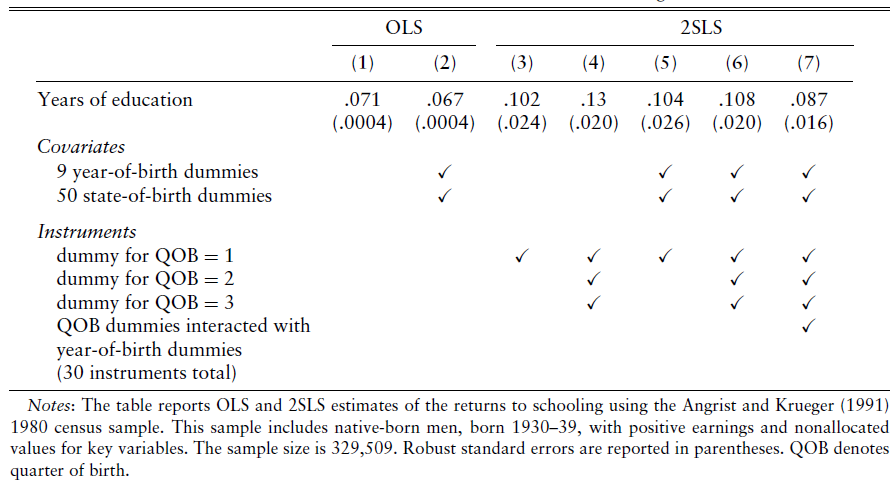
\includegraphics[scale=0.5]{./lecture_includes/ak_table.png}


\end{frame}

\begin{frame}{2SLS is a Many-Splendored Thing}

There is another (I think more useful) way to understand 2SLS: \\ as a weighted average of just-identified IVs:
\begin{align*}
\beta^{2SLS}&=\left(\pi^\prime Cov(\tilde{Z}_i,X_i^\prime)\right)^{-1} \pi^\prime Cov(\tilde{Z}_i,Y_i)\\
&=(\pi^\prime Var(\tilde{Z}_i)\pi)^{-1}\pi^\prime Var(\tilde{Z}_i)\rho,
\end{align*}
This is the formula for a $Var(\tilde{Z}_i)$-weighted regression of reduced- form coefficients $\rho$ on first-stage coefficients $\pi$ (with no constant)\pause{}
\begin{itemize}
\item When $J=1$ (one treatment), this becomes $\beta^{2SLS}=\sum_\ell \omega_\ell \beta_\ell^{IV}$ where $\omega_\ell=(\pi^\prime Var(\tilde{Z}_i)\pi)^{-1}\pi^\prime Var(\tilde{Z}_i)^\prime_\ell\pi_\ell$ and $\beta^{IV}_\ell = \rho_\ell/\pi_\ell$
\item Intuitively: 2SLS combines multiple ``one-at-a-time'' IVs $\beta_\ell^{IV}$
\end{itemize}

\end{frame}

\begin{frame}{Angrist-Hull '23: ``Visual IV'' for Cancer Screening Trials}
\begin{center}
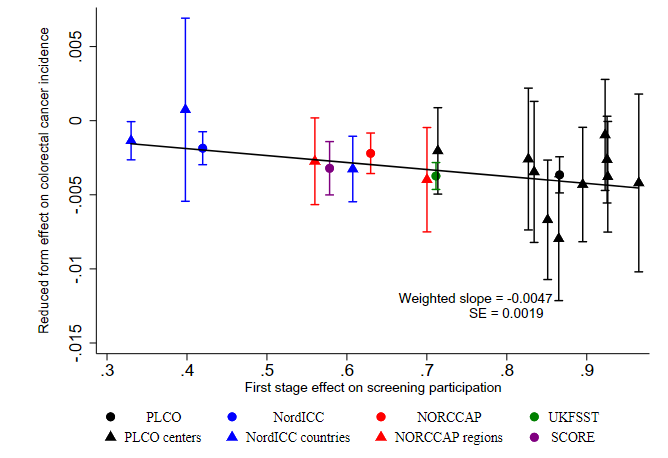
\includegraphics[scale=0.5]{./lecture_includes/pragmaticTrials.png}
\vspace{-0.3cm}
\end{center}
Each dot gives a ($\rho_\ell,\pi_\ell$) for a trial $\ell$ where  randomized screening offers $Z_i$ instrument for screening participation $D_i$
\begin{itemize}
\item Slope of the weighted line-of-best fit through zero = 2SLS estimate
\end{itemize}
\end{frame}

\begin{frame}{Overidentification Tests}

Under the constant-effects causal model of $Y_i=X_i^\prime\beta+\varepsilon_i$, overidentification gives a way to test instrument validity
\begin{itemize}
\item All just-identified IVs should coincide: i.e. $\beta_\ell^{IV}=\beta$ for all $\ell$
\item Graphically: the $R^2$ from visual IV plots should $= 1$ in large samples
\end{itemize}\medskip\pause{}
Stata will automatically give you the $p$-value for this test when $L>J$
\begin{itemize}
\item If $p>0.05$, it means your $\hat{\beta}_\ell^{IV}$'s are all pretty similar to each other
\end{itemize}\medskip\pause{}
Don't place too much stock in overidentification tests, however:
\begin{itemize}
\item They tend to have low power (b/c individual $\hat{\beta}_\ell^{IV}$ tend to be noisy)
\item If they reject, it need not mean your instruments are invalid \\ (b/c of treatment effect heterogeneity -- more on this soon)
\item Rejection doesn't tell you which IV is invalid (they all might be!)
\end{itemize}
\end{frame}

\subsection{Weak vs. Many-Weak Bias}

\begin{frame}{Weak Instruments}
\vspace{-0.2cm}

When running just-identified IV, people worry about instrument ``strength'' \vspace{-0.7cm}
\begin{itemize}
  \item Specifically the first stage F-statistic, which tests if $\pi=0$ 
\end{itemize}
\smallskip\pause

If $\pi$ is small relative to its standard error, we say the IV is ``weak''
\begin{itemize}
  \item Typically use the rule-of-thumb of $F<10$ (Staiger and Stock 1997)
  \item In this case the second-stage SEs will be large and the 2SLS estimate will tend to be biased towards the corresponding OLS
\end{itemize}\pause

Much has been made of this over the years, but Angrist and Koles\'{a}r (2022) show that we shouldn't worry too much
\begin{itemize}
  \item The SE increase tends to be large enough to ``cover up'' the bias, \\ so you're unlikely to reject the null of $\beta=0$ spuriously 
\end{itemize}

\end{frame}

\begin{frame}{Weak Instruments: Visualized}
\vspace{-0.2cm}
Monte Carlo: $Y_i=0\cdot D_i + \varepsilon_i$, $D_i=\pi Z_i+\eta_i$: $\pi=Var(\varepsilon_i)=Var(\eta_i)=1$
\begin{center}
\includegraphics[scale=0.45]{./lecture_includes/strongpi.png}
\end{center}

\end{frame}

\begin{frame}{Weak Instruments: Visualized}
\vspace{-0.2cm}
Monte Carlo: $Y_i=0\cdot D_i + \varepsilon_i$, $D_i=\pi Z_i+\eta_i$: $\pi=0.1$ (Weaker)
\begin{center}
\includegraphics[scale=0.35]{./lecture_includes/medpi.png}
\end{center}

\end{frame}

\begin{frame}{Weak Instruments: Visualized}
\vspace{-0.2cm}
Monte Carlo: $Y_i=0\cdot D_i + \varepsilon_i$, $D_i=\pi Z_i+\eta_i$: $\pi=0.01$ (Very Weak)
\begin{center}
\includegraphics[scale=0.35]{./lecture_includes/weakpi.png}
\end{center}

\end{frame}

\begin{frame}{Many IVs}
\vspace{-0.2cm}
A thornier problem is many-weak bias, when overidentified\smallskip
\begin{itemize}
\item This also tends to manifest in low first-stage F's, and also causes 2SLS to be biased towards OLS
\end{itemize}\bigskip\pause{}

Unlike when just-id., however, with many weak IVs the SE's go \emph{down}\smallskip
\begin{itemize}
  \item Intuitively, a more flexible FS tends to fit $D_i$ better $\rightarrow$ more power\smallskip
  \item But we can have \emph{overfitting} with lots of instruments, which essentially recreates the (endogenous) variation in $D_i$ 
\end{itemize}\bigskip\pause{}

This became a high-profile problem with Angrist-Krueger ‘91, where the QOB
instrument was interacted with many state/year FEs
\smallskip
\begin{itemize}
  \item These days folks don’t make this mistake ... but many-IV bias can be
lurking in other settings with constructed instruments (e.g. judge IV)
\end{itemize}

\end{frame}

\begin{frame}{Many Instruments: Visualized}
\vspace{-0.2cm}
$Y_i=0\cdot D_i + \varepsilon_i$, $D_i=\pi Z_{i1}+\sum_{\ell>1} 0\cdot Z_{i\ell}+\eta_i$: IV w/ $Z_{i1}$ only
\begin{center}
\includegraphics[scale=0.35]{./lecture_includes/fewz.png}
\end{center}

\end{frame}

\begin{frame}{Many Instruments: Visualized}
\vspace{-0.2cm}
$Y_i=0\cdot D_i + \varepsilon_i$, $D_i=\pi Z_{i1}+\sum_{\ell>1} 0\cdot Z_{i\ell}+\eta_i$: IV w/ $Z_{i1},\dots,Z_{i10}$
\begin{center}
\includegraphics[scale=0.35]{./lecture_includes/somez.png}
\end{center}

\end{frame}

\begin{frame}{Many Instruments: Visualized}
\vspace{-0.2cm}
$Y_i=0\cdot D_i + \varepsilon_i$, $D_i=\pi Z_{i1}+\sum_{\ell>1} 0\cdot Z_{i\ell}+\eta_i$: IV w/ $Z_{i1},\dots,Z_{i100}$
\begin{center}
\includegraphics[scale=0.35]{./lecture_includes/manyz.png}
\end{center}

\end{frame}

\begin{frame}{What to Do?}
\vspace{-0.2cm}
Aim for few instruments, and check your F's after every \emph{ivreg}\smallskip
\begin{itemize}
\item State of the art: Montiel Olea and Pflueger '15; \code{weakivtest} in Stata\smallskip
\item Staiger-Stock rule-of-thumb ($F>10$) still seems widely held\smallskip
\item See Lee et al. (2020) and Keane and Neal (2022) for some discussions of additional subtleties
\end{itemize}
\medskip\pause{}

If your F is small, some things to consider:\smallskip
\begin{itemize}
\item Is there a better functional form for your instrument?\smallskip
\item Do interactions with covariates help? (note: beware many-weak!)\smallskip
\item Does changing the covariate set help? (note: beware invalidity!)\smallskip
\item Check results w/a more robust approach (e.g. Anderson-Rubin, JIVE)
\end{itemize}


\end{frame}

\section{IV Interpretation}

\subsection{LATE and Generalizations}

\begin{frame}{What Does IV Identify, Really?}

IV was invented in the context of structural economic models, typically with a single parameter $\beta$ linearly relating $Y_i$ to $X_i$ 
\begin{itemize}
\item These days we understand $Y_i=\beta X_i+\varepsilon_i$ as describing a \emph{causal} relationship, imposing a (strong) constant-effects restriction
\end{itemize} \pause{}\medskip

The Imbens-Angrist LATE result revolutionized our understanding of IV estimands, and clarified some subtle points around IV identification
\begin{itemize}
\item $\beta^{IV}$ often identifies a convex average of heterogeneous effects under first-stage \emph{monotonicity}: $Z_i$ only affects $X_i$ in one direction
\item IV ``exogeneity'' can arise from two conceptually different assumptions of instrument \emph{independence} and \emph{exclusion}
\end{itemize}
\end{frame}

\begin{frame}{Basic (Binary Treatment, Binary Instrument) Setup}
Let $Y_i(0)$ and $Y_i(1)$ denote individual $i$'s potential outcomes given a binary treatment $D_i\in\{0,1\}$\smallskip
\begin{itemize}
\item Observed outcomes: $Y_i=\left(Y_i(1)-Y_i(0)\right)D_i+Y_i(0)\pause{}\equiv\beta_i D_i+\varepsilon_i$
\end{itemize}\medskip\pause{}
Let $D_i(0)$ and $D_i(1)$ denote individual $i$'s potential treatment given a binary instrument $Z_i\in\{0,1\}$\smallskip
\begin{itemize}
\item Observed treatment: $D_i=\left(D_i(1)-D_i(0)\right)Z_i+D_i(0)$
\end{itemize}\medskip\pause{}
Under what assumptions can we causally interpret \code{ivreg2 Y (D=Z)}?
\end{frame}

\begin{frame}{Imbens and Angrist (1994) Assumptions}
\begin{enumerate}
\item \emph{As-good-as-random assignment}: $Z_i\perp (Y_i(0),Y_i(1),D_i(0),D_i(1))$\smallskip
\begin{itemize}
\item Consider the Angrist draft lottery, or Angrist-Krueger's QoB IV
\end{itemize}\medskip\pause{}
\item \emph{Exclusion}: $Z_i$ only affects $Y_i$ through its effect on $D_i$\smallskip
\begin{itemize}
\item Implicit in the potential outcome notation: $Y_i(d)$ is not indexed by $Z_i$
\end{itemize}\medskip\pause{}
\item \emph{Relevance}: $Z_i$ is correlated with $D_i$\smallskip
\begin{itemize}
\item Equivalently, given Assumption 1, $E[D_{i}(1)-D_i(0)]\neq 0$
\end{itemize}\medskip\pause{}
\item \emph{Monotonicity}: $D_{i}(1)\ge D_{i}(0)$ for all $i$ (i.e., almost-surely)\smallskip
\begin{itemize}
\item The instrument can only shift the treatment in one direction
\end{itemize}
\end{enumerate}
\end{frame}

\begin{frame}{Local Average Treatment Effect (LATE) Identification}
Imbens and Angrist showed that under these assumptions:
\begin{align*}
\beta^{IV}=E[Y_i(1)-Y_i(0)\mid D_i(1)>D_i(0)]
\end{align*}
\vspace{-0.6cm}

The IV estimand $\beta^{IV}$ identifies a LATE: the average treatment effect $Y_i(1)-Y_i(0)$ among \emph{compliers}: those with $1=D_i(1)>D_i(0)=0$\smallskip\pause{}
\begin{itemize}
\item Intuitively, IV can't tell us anything about the treatment effects of \emph{never-takers} $D_i(1)=D_i(0)=0$ or \emph{always-takers} $D_i(1)=D_i(0)=1$\smallskip\pause{}
\item Monotonicity rules out the presence of \emph{defiers}, with $D_i(1)<D_i(0)$
\end{itemize}
\end{frame}

\imageframe{./lecture_includes/angrist_1990.png}

\begin{frame}{What Does This Mean \emph{Practically}?} 
Two conceptually distinct considerations: \emph{internal} vs. \emph{external} validity\smallskip
\begin{itemize}
\item Context of an IV, and who the compliers likely are, may matter\smallskip
\item Usual ``overidentification'' test logic fails: two valid IVs may have different estimands
\end{itemize}\medskip\pause{}
In addition to as-good-as-random assignment / exclusion, we may need to worry about monotonicity when we do IV\smallskip
\begin{itemize}
\item Sensible in many settings (e.g. draft lottery / cancer screening RCTs) \smallskip
\item Maybe questionable in judge IVs (see Eric's earlier slides)
\end{itemize}\medskip\pause{}

Note: technically, we don't need monotonicity if effects are homogenous
\end{frame}

\begin{frame}{Generalizations and Limitations}

\vspace{-0.2cm}
The core logic of IA'94 extends to multivalued treatments/instruments
\begin{itemize}
\item IV identifies an avg. of incremental treatment effects, putting more weight on margins where the instrument shifts the treatment more
\item Regressions of $\mathbf{1}[X_i\ge x]$ on $Z_i$ identify the weights
\end{itemize}\medskip\pause{}
The result does \emph{not} easily extend, however, to multiple treatments 
\begin{itemize}
\item Contamination bias: IV coefficient on $X_{ij}$ generally incorporates effects from other treatments $X_{ik}$, $k\neq j$ 
\end{itemize}\medskip\pause{}
Since 2SLS is a weighted average of ``one-at-a-time'' IVs, overidentified single-treatment specifications can have a LATE interpretation
\begin{itemize}
\item Need all individual IVs to have a LATE interpretation and the 2SLS weights to be convex (the latter can be checked empirically)
\end{itemize}
\end{frame}

\begin{frame}{Generalizations and Limitations (Cont.)}

We can also have a LATE interpretation in IV specifications w/controls
\begin{itemize}
\item E.g. if $Z_i$ is only as-good-as-randomly assigned conditional on $W_i$
\end{itemize}\medskip\pause{}

Key condition: the controls are flexible enough to make $E[Z_i\mid W_i]$ linear
\vspace{-0.7cm}
\begin{itemize}
\item E.g. $W_i$ is a set of mutually exclusive strata dummies
\item IV then identifies a weighted-average of conditional-on-$W_i$ IVs
\end{itemize}\medskip\pause{}

If $E[Z_i\mid W_i]$ is nonlinear, IV may be biased (even w/constant effects)
\begin{itemize}
\item Key practical takeaway: it's good to check sensitivity to how controls are parameterized (add interactions, higher-order polynomials, etc.)
\end{itemize}
\end{frame}

\subsection{Characterizing Compliers}

\begin{frame}{Who Are the Compliers?}
Characterizing the $i$ that make up the IV estimand (w/$D_i(1)>D_i(0)$) is key for understanding internal vs. external validity \smallskip
\begin{itemize}
\item Unfortunately we can't identify compliers directly: we only observe $D_i(1)$ (when $Z_i=1$) or $D_i(0)$ (when $Z_i=0$), not both together!
\end{itemize}\bigskip\pause{}
As it turns out, we can still characterize compliers by their outcomes ($Y_i(0)$ and $Y_i(1)$) and by other observables $X_i$\smallskip
\begin{itemize}
\item Comparing $E[X_i\mid D_i(1)>D_i(0)]$ to $E[X_i]$ can maybe shed light on how $E[Y_i(1)-Y_i(0)\mid D_i(1)>D_i(0)]$ compares to $E[Y_i(1)-Y_i(0)]$
\end{itemize}
\end{frame}


\begin{frame}{Outcomes}
Computing $E[Y_i(1)\mid D_i(1)>D_i(0)]$ is surprisingly easy in the IA setup\smallskip
\begin{itemize}
\item Define $W_i=Y_iD_i$, and note that this new outcome has potentials with respect to $D_i$ of $W_i(1)=Y_i(1)$ and $W_i(0)=0$\smallskip\pause{}
\item Thus IV with $W_i$ as the outcome identifies $E[W_i(1)-W_i(0)\mid D_i(1)>D_i(0)]=E[Y_i(1)\mid D_i(1)>D_i(0)]$
\end{itemize}\medskip\pause{}
Similar logic shows that IV with $Y_i(1-D_i)$ as the outcome and $1-D_i$ as the treatment identifies $E[Y_i(0)\mid D_i(1)>D_i(0)]$\smallskip
\begin{itemize}
\item So easy to do! And extends to covariates / multiple IVs...
\end{itemize}
\end{frame}

\begin{frame}{Illustration: Angrist et al. (2013) Charter School IV}

\begin{center}
	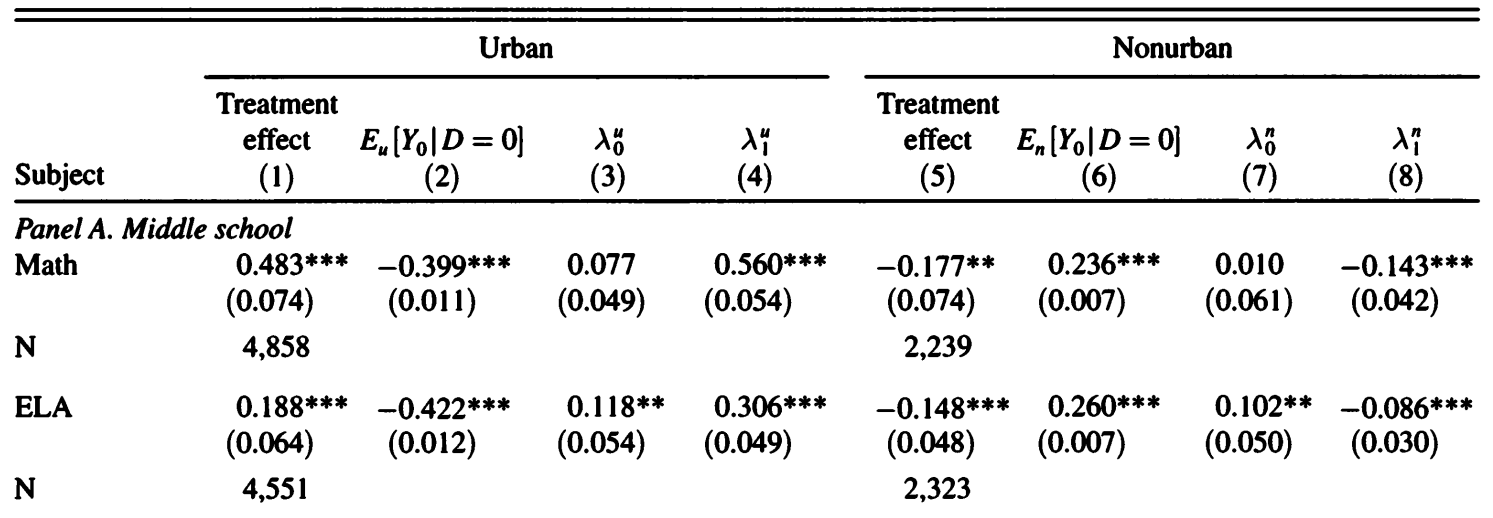
\includegraphics[width=1\textwidth]{./lecture_includes/apw_2013.png}
\end{center}
Decomposing
\vspace{-0.5cm}
\begin{align*}
LATE=&\underbrace{E[Y_i(1)\mid D_i(1)>D_i(0)]-E[Y_i(0)\mid D_i=0]}_{\lambda_1} \\
&- \underbrace{(E[Y_i(0)\mid D_i(1)>D_i(0)]-E[Y_i(0)\mid D_i=0])}_{\lambda_0}
\end{align*}
\vspace{-0.7cm}

shows that charter compliers have typical counterfactual achievement

\end{frame}


\vspace{-0.5cm}
\begin{frame}{Covariates}
For covariates $X_i$ (not affected by $D_i$) we can follow a similar trick:
\begin{itemize}
\item Either IV'ing $X_iD_i$ on $D_i$ or IV'ing $X_i(1-D_i)$ on $1-D_i$ identifies complier characteristics $E[X_i\mid D_i(1)>D_i(0)]$\smallskip
\item Shouldn't be very different (implicit balance test); can be averaged
\end{itemize}\bigskip\pause{}
Can be useful to compare with always- and never-taker means:
\begin{itemize}
\item AT: $E[X_i\mid D_i(1)=D_i(0)=1]=E[X_i\mid D_i=1,Z_i=0]$\smallskip
\item NT: $E[X_i\mid D_i(1)=D_i(0)=0]=E[X_i\mid D_i=0,Z_i=1]$
\end{itemize}
\end{frame}

\begin{frame}{Illustration: Angrist et al. (2023) Charter School IV}

\vspace{-0.2cm}
\begin{center}
	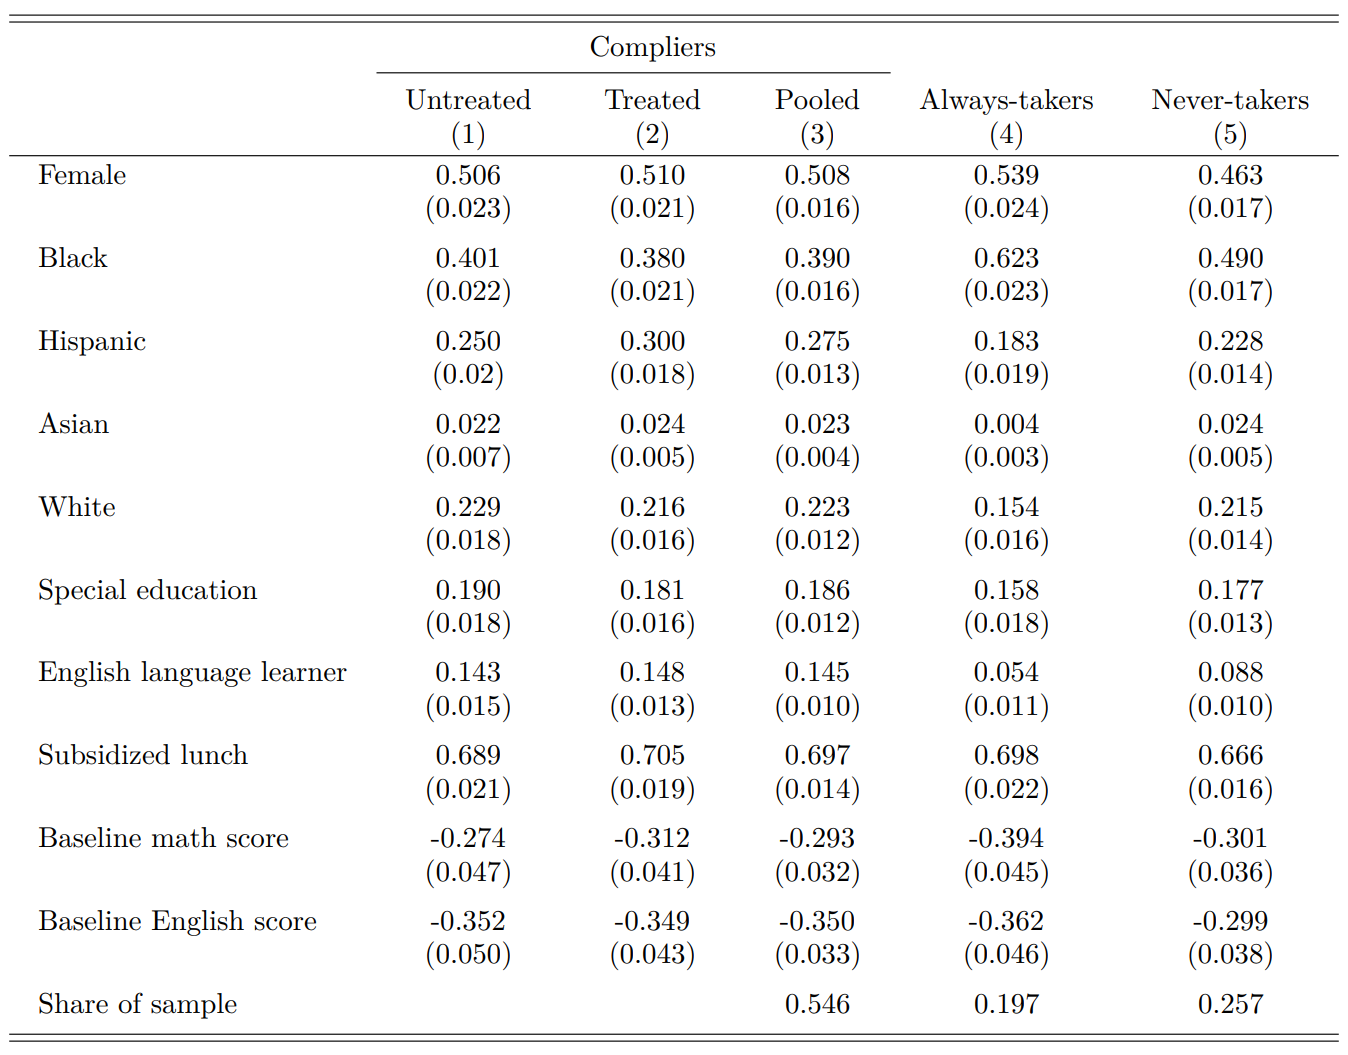
\includegraphics[width=0.9\textwidth]{./lecture_includes/hoee_characteristics.png}
\end{center}

\end{frame}

\begin{frame}{Fancier Things}

General result: $E[g(X_i,Y_i(d))\mid D_i(1)>D_i(0)]$ for any $g(\cdot)$ and any $d\in\{0,1\}$ is identified by $\beta$ in the IV regression:
\begin{align*}
g(X_i,Y_i)\times \mathbf{1}[D_i=d]&=\alpha + \beta\mathbf{1}[D_i=d] + \varepsilon_i\\
\mathbf{1}[D_i=d]&= \mu + \pi Z_i + \nu_i
\end{align*}\pause{}
\vspace{-0.5cm}

Lots of fun stuff we can do here. E.g.: distributions\smallskip
\begin{itemize}
\item $g(X_i,Y_i)=\mathbf{1}[Y_i\le y]$ estimates the CDF of complier potential outcomes, $F(y)=Pr(Y_i(d)<y\mid D_i(1)>D_i(0))$\smallskip
\item $g(X_i,Y_i)=\frac{1}{h}K(\frac{Y_i-y}{h})$ estimates the corresponding PDF, where $K(\cdot)$ is a kernel function and $h$ is a bandwidth 
\end{itemize}

\end{frame}

\begin{frame}{Illustration: Angrist et al. (2023) Charter School IV}
\vspace{-0.2cm}
\begin{center}
	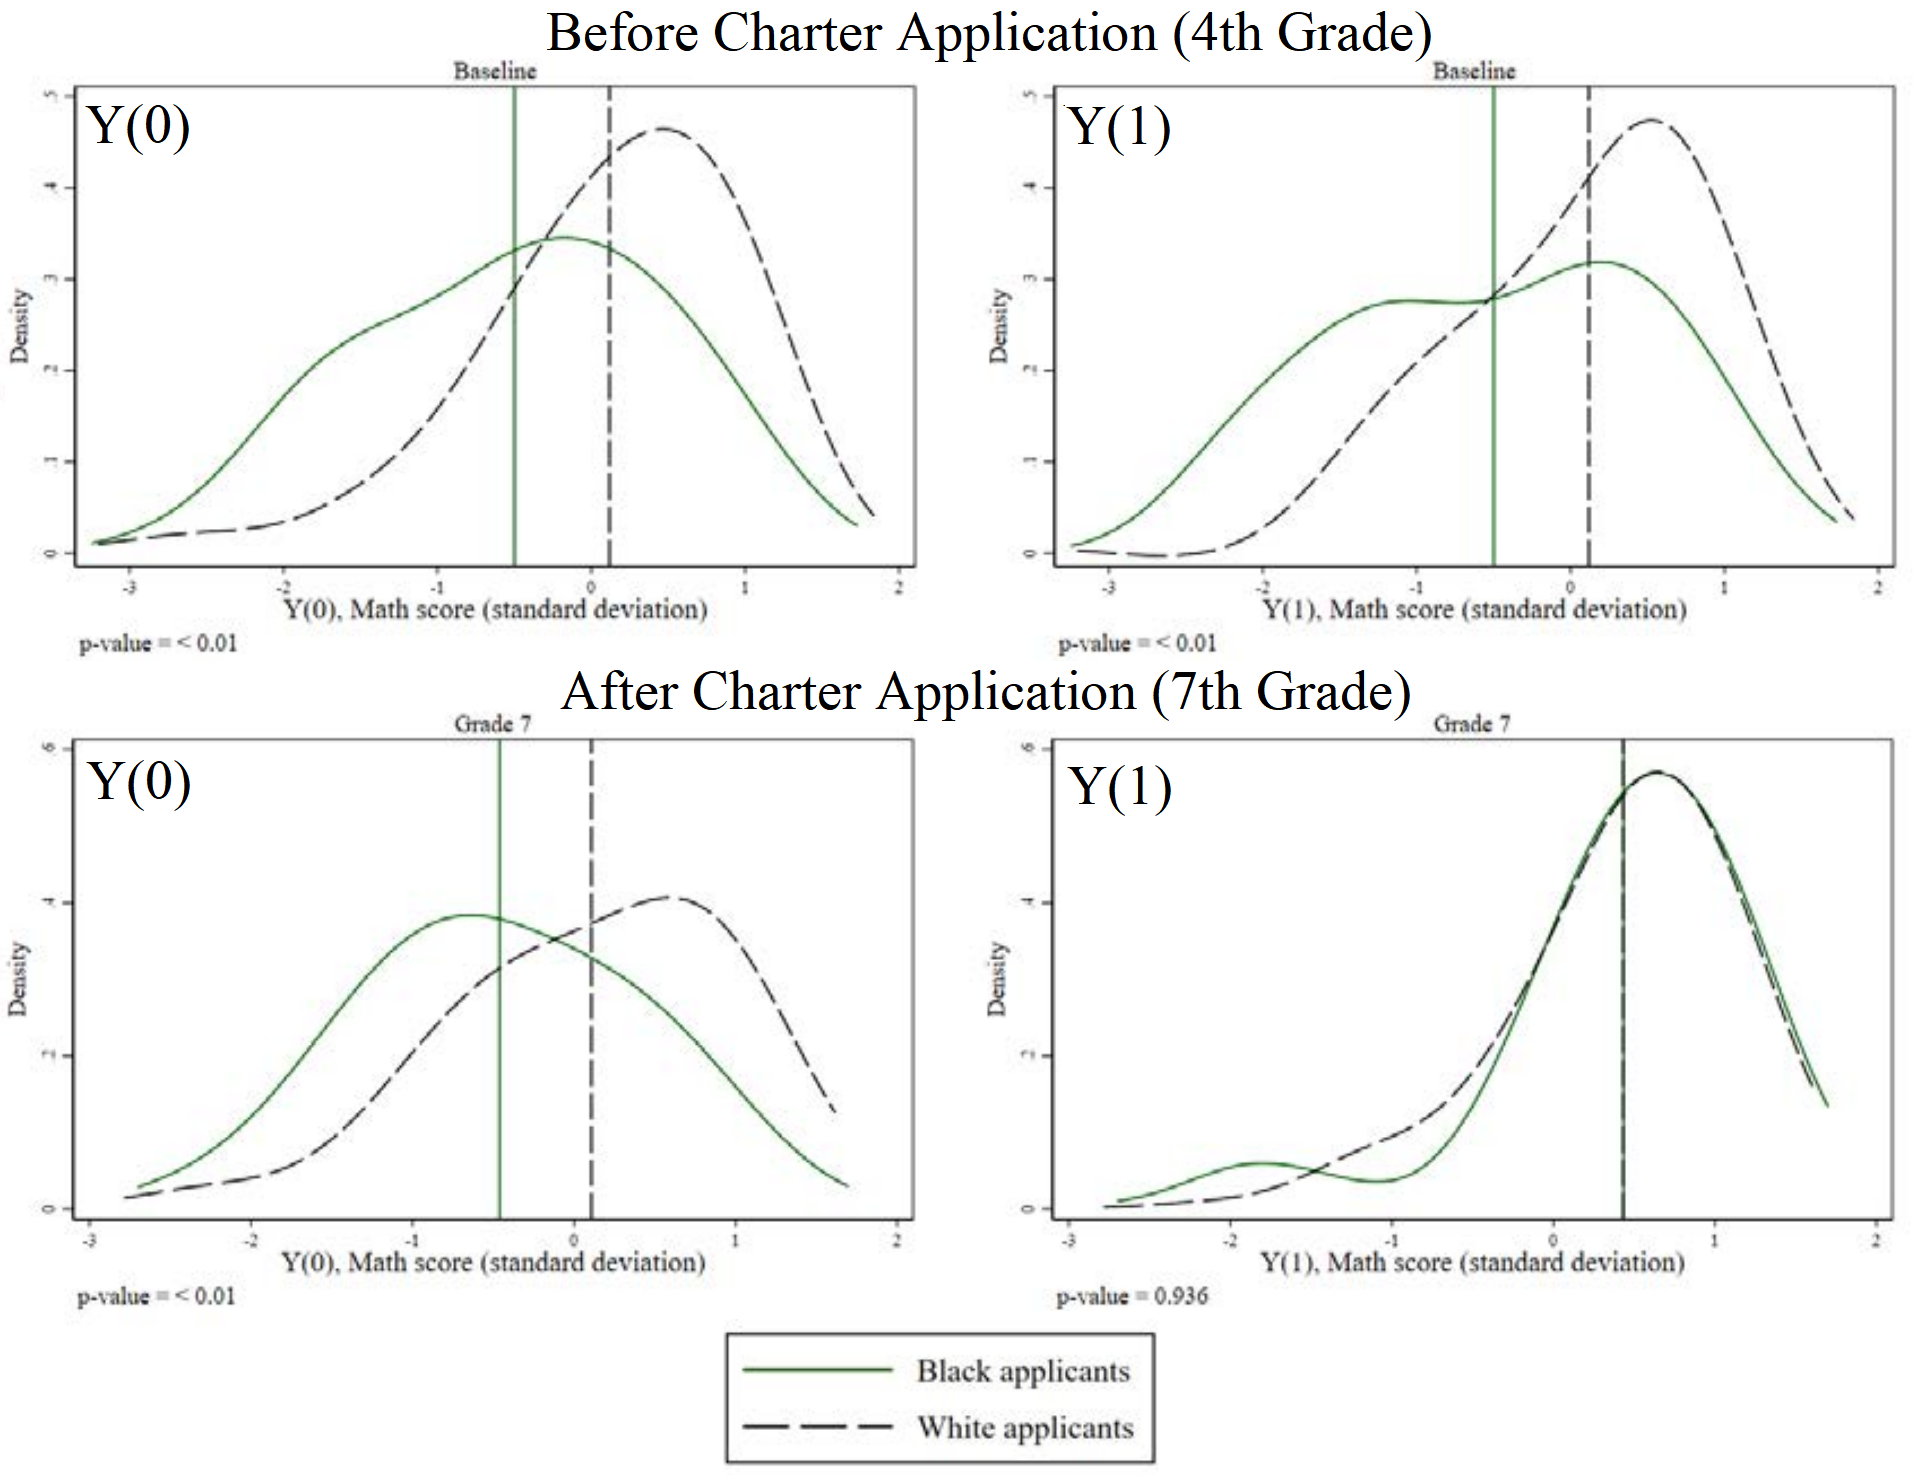
\includegraphics[width=0.9\textwidth]{./lecture_includes/hoee_distribution.png}
\end{center}
\end{frame}

\begin{frame}{Outside the Basic IA Setup}

The same logic applies to IV regressions with flexible controls \smallskip
\begin{itemize}
\item E.g. \emph{ivreg}ing $Y_iD_i$ on $D_i$ instrumenting by $Z_i$ and controlling for cell FE ID's a weighted avg of within-cell $E[Y_i(1)\mid D_i(1)>D_i(0)]$\smallskip\pause{}
\item Abadie (2003) ``kappa-weighting'' is an alternative approach for unweighted averages (and other things)
\end{itemize}\bigskip\pause{}

Logic also goes through with continuous instruments\smallskip
\begin{itemize}
\item E.g. can always mechanically decompose an IV on a binary $D_i$ into implied ``$Y(1)$'' and ``$Y(0)$'' terms
\item Unfortunately, things get trickier with non-binary treatments
\end{itemize}

\end{frame}

\subsection{Diff-in-Diff and IV}

\begin{frame}{What about Diff-in-Diff?}
Most LATE-style discussions of IV identification are ``design-based'': \\ i.e., the instrument is assumed to be drawn randomly, as if in an RCT 
\begin{itemize}
\item But not all instruments are easily thought of this way (e.g. distance)
\end{itemize}\medskip\pause{}

Luckily, whenever you have a reduced form \& first stage that are causal and exclusion+monotonicity hold, the IV ratio has a LATE interpretation
\begin{itemize}
\item E.g. diff-in-diff IV, for distance measure $Z_i\in\{0,1\}$ and $t\in\{1,2\}$:
\vspace{-0.4cm}
\begin{align*}
Y_{it}&=\alpha_i + \tau_t + \beta D_{it} + \epsilon_{it} \\
D_{it}&=\mu_i + \lambda_t + \pi Z_{i}\times\mathbf{1}[t=2] + \epsilon_{it}
\end{align*}
\vspace{-1cm}

Parallel trends in $Z_i$ make the reduced form \& first stage causal\pause{}
\item Recent TWFE literature becomes relevant with fancier specifications
\end{itemize}
\end{frame}

\begin{frame}{Example: Duflo (2001) School-Building Diff-in-Diff}
\begin{center}
	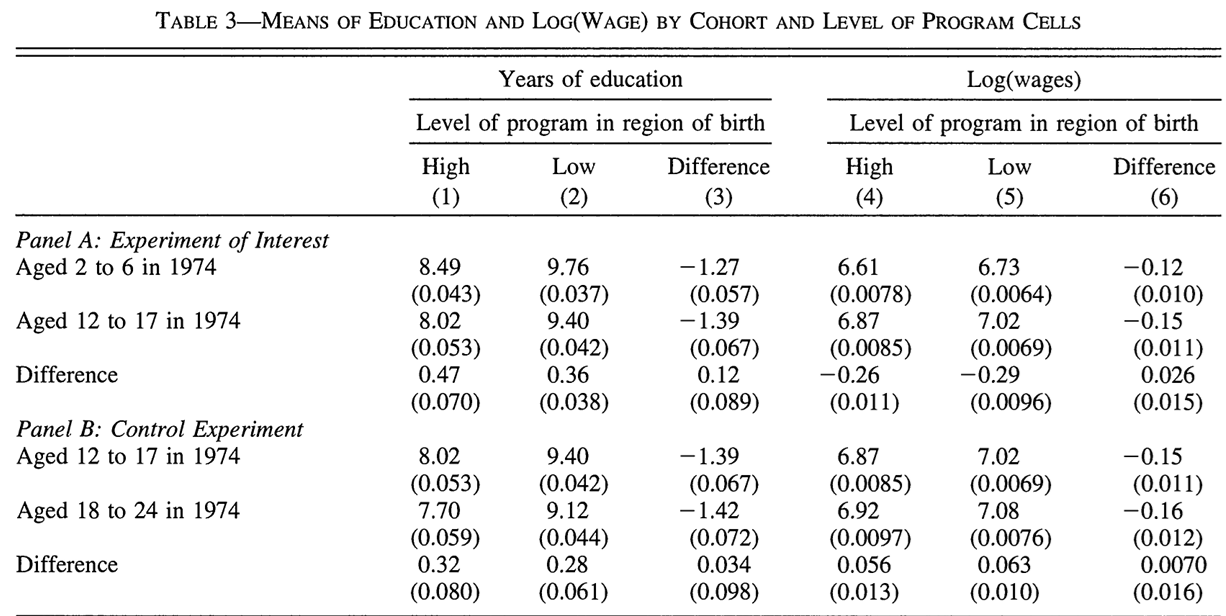
\includegraphics[width=1\textwidth]{./lecture_includes/duflo_2001.png}
\end{center}
Here $Z_i=$ growing up in a region with intensive school building
\end{frame}
\section{Formula Instruments}

\begin{frame}{Exogenous Shocks with Non-Random Exposure}
Increasingly, researchers construct instruments from multiple sources of variation --- only some of which is viewed as exogenous. E.g.:
\begin{itemize}
\item Shift-share instruments $Z_i=\sum_k s_{ik}g_k$, which average together a set of shocks $g_k$ with predetermined exposure shares $s_{ik}$
\item IVs capturing spillovers across social networks/geographies 
\item ``Simulated'' instruments, capturing eligibility for a public program
\end{itemize}\medskip\pause{}

Generically, $Z_i=f_i(g,s)$ where $g=(g_1,\dots,g_k)$ is a set of shocks, $s$ is some measure of shock exposure, and $f_i(\cdot)$ is a known formula
\begin{itemize}
\item How can we leverage exogeneity in $g$, allowing $s$ to be non-random?
\end{itemize}

\end{frame}

\subsection{Shift-Share IV}

\begin{frame}{Example: Autor, Dorn, and Hanson (2014)}
ADH study the effects of rising Chinese import competition on US commuting zones in the 1990's and 2000's
\begin{itemize}
\item Treatment $X_{i}$: growth of Chinese imports in CZ $i$
\item Main outcome $Y_{i}$: change in manufacturing employment in CZ $i$
\end{itemize}\medskip\pause{}

They use a shift-share instrument $Z_{i}=\sum_k s_{ik}g_{k}$, where:
\begin{itemize}
\item Shocks $g_k$: industry $k$'s Chinese import growth in non-US economies
\item Shares $s_{ik}$: pre-period employment share of industry $k$ in CZ $i$
\end{itemize}\medskip\pause{}

Idea: $Z_i$ predicts $X_i$ with proxies for underlying productivity shocks  
\begin{itemize}
\item Fairly intuitive ... but what do we need for it to work? 
\end{itemize}
\end{frame}

\begin{frame}{SSIV with Exogneous Shocks}

Borusyak, Hull, and Jaravel (2022) show shift-share IV can work when
\begin{itemize}
\item The shocks $g_k$ are exogenous, at least conditional on some $q_k$
\item There is enough independent variation in the shocks (i.e. large $K$)
\end{itemize}\bigskip\pause{}

Intuitively, $Z_i=\sum_k s_{ik}g_{k}$ works as a ``translation device,'' bringing the $k$-level variation to bear on causal effects at the $i$ level
\begin{itemize}
\item E.g. in Autor et al. (2014), an industry-level natural experiment can be used to estimate effects at the commuting zone level
\item The shares $s_{ik}$ used for this translation do not need to be exogenous!
\end{itemize}

\end{frame}

\begin{frame}{Two Practical Considerations}

Need to control for $E[Z_i\mid s,q]=E[\sum_k s_{ik}g_{k}\mid s,q]=\sum_k s_{ik}E[g_k\mid q]$ \\ in order to isolate the as-good-as-random variation in shocks
\begin{itemize}
\item When $E[g_k\mid q]=q_k^\prime\gamma$, this means controlling for $\sum_k s_{ik}q_k$ 
\item E.g. in Autor et al. (2014), to isolate within-period shock variation, need to control for $\sum_k s_{ik}\times (\text{period FE})$
\end{itemize}\bigskip\pause{}

Need to adjust SEs for a non-standard clustering: $Z_i=\sum_k s_{ik}g_k$ and $Z_j=\sum_k s_{jk} g_k$ are correlated via their common exposure to shocks
\begin{itemize}
\item Easy fix: use the \emph{ssaggregate} Stata/R packages to translate SSIV estimation to the level of identifying variation (shocks)
\end{itemize}
\end{frame}

\begin{frame}{Estimating Exogenous-Shock SSIV Regressions in Stata}
\vspace{-0.3cm}
\begin{center}
\includegraphics[scale=0.27]{./lecture_includes/ssaggregate.png}
\end{center}
To install: \code{ssc install ssaggregate}
\end{frame}

\begin{frame}{Autor et al. (2014) Revisited}
\begin{center}
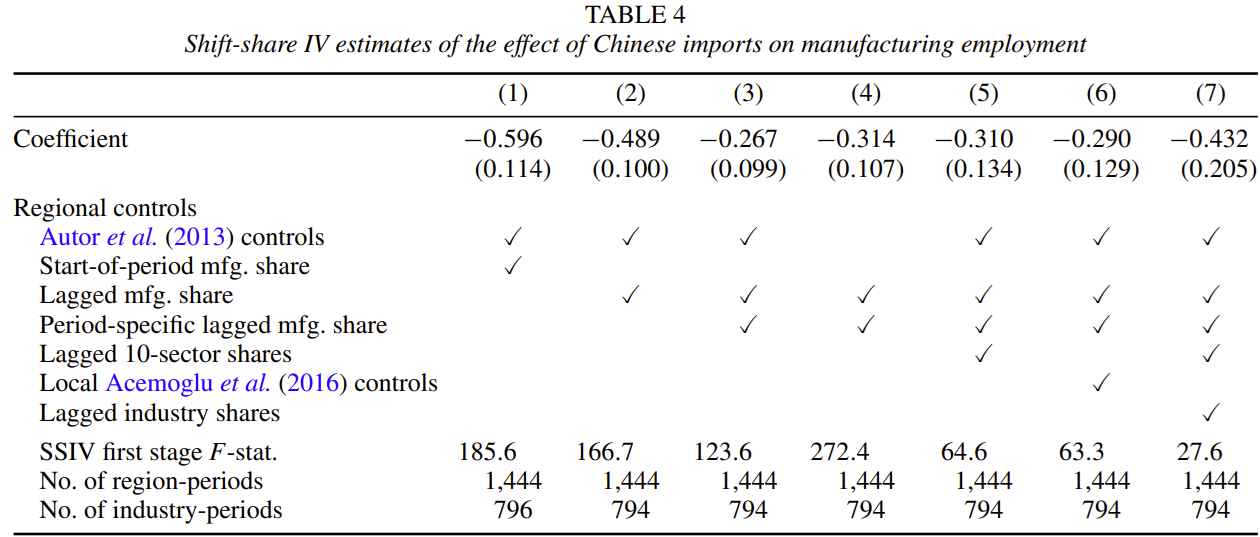
\includegraphics[scale=0.52]{./lecture_includes/adh_bhj_restud.png}
\end{center}
\begin{itemize}
\item Columns 3-7 include the key  $\sum_k s_{ik}\times (\text{period FE})$ control
\item Standard errors / first stage F-stat.'s computed via \emph{ssaggregate}
\end{itemize}
\end{frame}

\subsection{Recentered IV}
\begin{frame}{Beyond Shift-Share}

Suppose we wanted to estimate the economic impact of new transportation upgrades (e.g. new high speed rail construction)
\begin{itemize}
\item Economic theory tells us to expect spillovers: easier travel increases productivity across all cities $i$ in a country, to different extents
\item E.g. \emph{market access}: $X_i=\sum_j \tau(g,loc_i,loc_j)^{-1}pop_j$ where $g$ captures the railroad network, $loc_i$ gives lat/lon of cities, and $pop_i$ is city size
\end{itemize}\bigskip\pause{}

Like a more complex shift-share: $Z_i=f_i(g,s)$ for $s=(loc_i,pop_i)_{i=1}^{N}$
\begin{itemize}
\item Suppose we had a natural experiment in high-speed rail construction; can we ``translate'' these $g$ shocks via the market access mapping?
\end{itemize}
\end{frame}

\begin{frame}{Recentered IV}

Borusyak and Hull (2023) show how to leverage exogenous $g$ in $f_i(g,s)$:
\begin{enumerate}
\item Specify \emph{counterfactual} exogenous shocks $g^{(1)},\dots,g^{(C)}$ which may well have occured (e.g. shuffle the timing of new rail construction)
\item Recompute the instrument: $Z_i^{(c)}=f_i(g^{(c)},s)$, for $c=1,\dots,C$
\item Take the average (``expected instrument''): $\mu_i=\frac{1}{C}\sum_i Z_i^{(c)}$
\end{enumerate}\bigskip\pause{}

Either controlling for $\mu_i$ or using the recentered $\tilde{Z}_i=Z_i-\mu_i$ avoids any bias from endogeneity/non-randomness in $Z_i$
\begin{itemize}
\item Analogous to controlling for $\sum_k s_{ik}q_k$ in shift-share IV! 
\item BH also discuss the analog of non-standard SSIV clustering:\\ the solution is a bit more non-standard (randomization inference)
\end{itemize}

\end{frame}

\begin{frame}[t]{Illustration: High-Speed Rail in China} 
\vspace{-0.3cm}
	\begin{center}
		149 lines were built or planned (as of April 2019)

		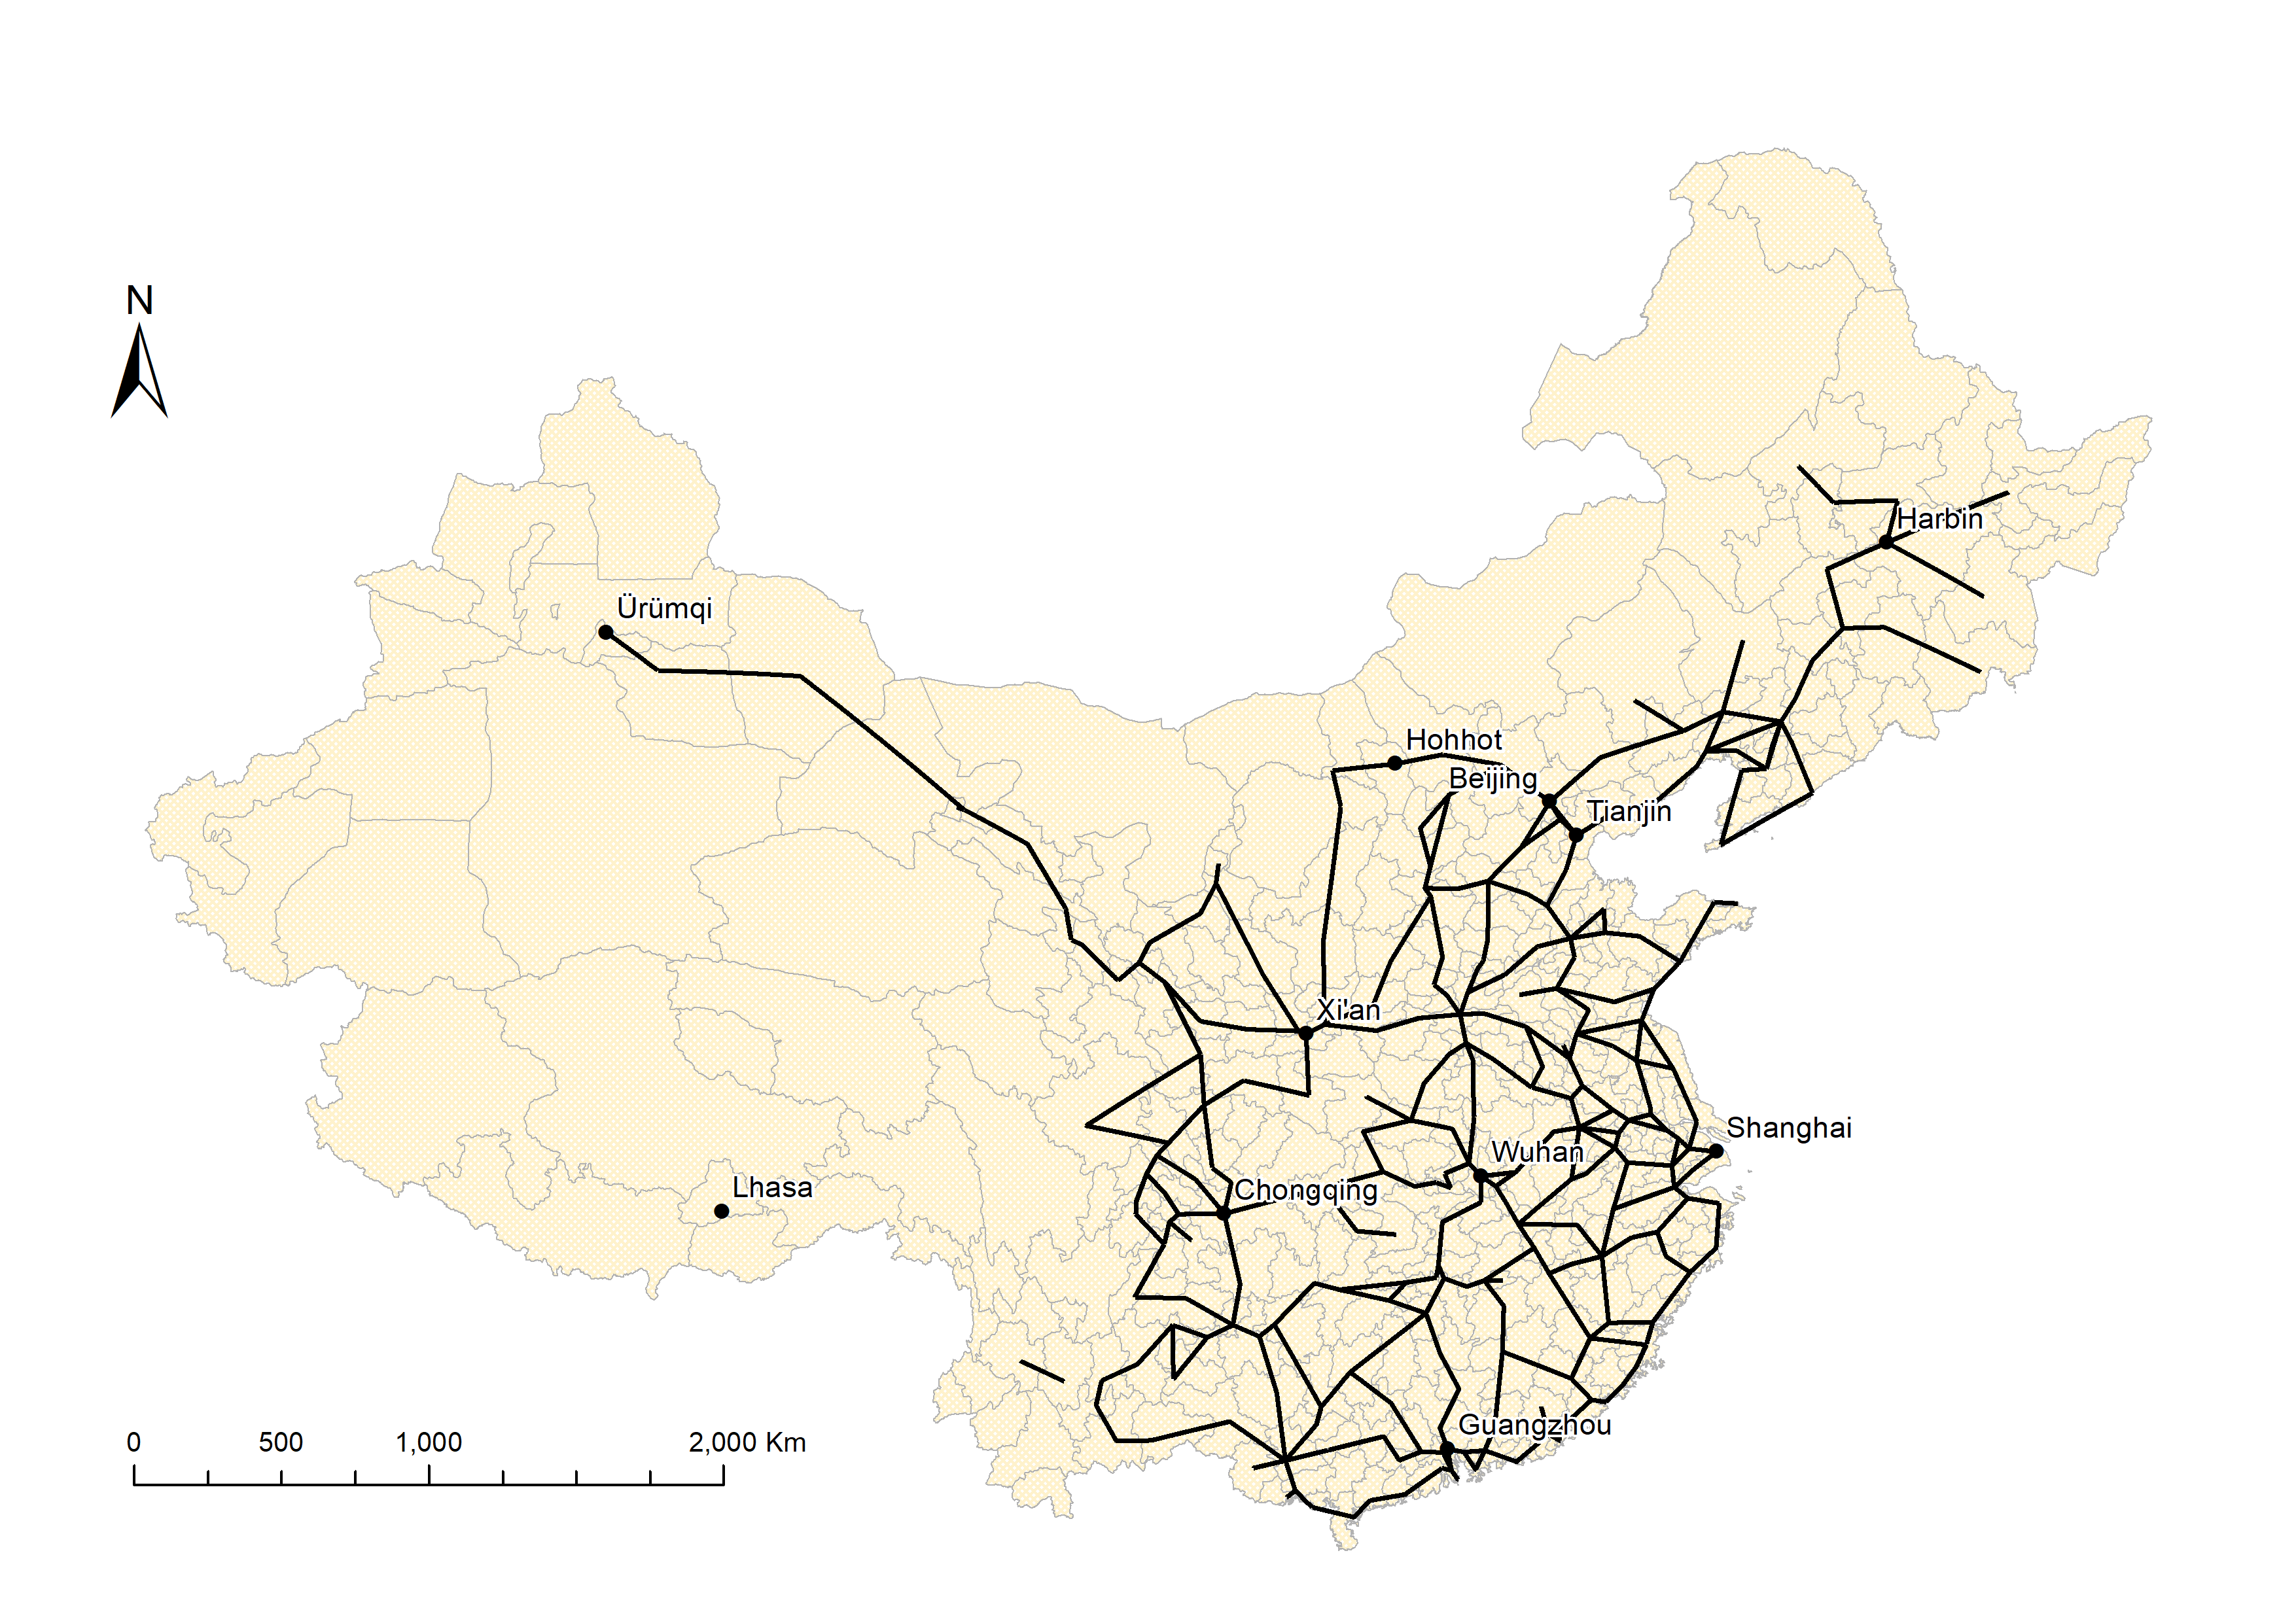
\includegraphics[trim={1cm 0.5cm 0.5cm 1cm},clip,width=11cm]{lecture_includes/Lines_actual_planned_nocolor.png}
	\end{center}
\end{frame}

\begin{frame}[t]{Illustration: High-Speed Rail in China} 
\vspace{-0.3cm}
	\begin{center}
		The 83 lines actually built by 2016. Suppose exact timing is random

		\includegraphics[trim={1cm 0.5cm 0.5cm 1cm},clip,width=11cm]{lecture_includes/Line_panel2016.png}
	\end{center}
\end{frame}

\begin{frame}[t]{Illustration: High-Speed Rail in China} 
\vspace{-0.3cm}
	\begin{center}
		A counterfactual draw of 83 lines by 2016

		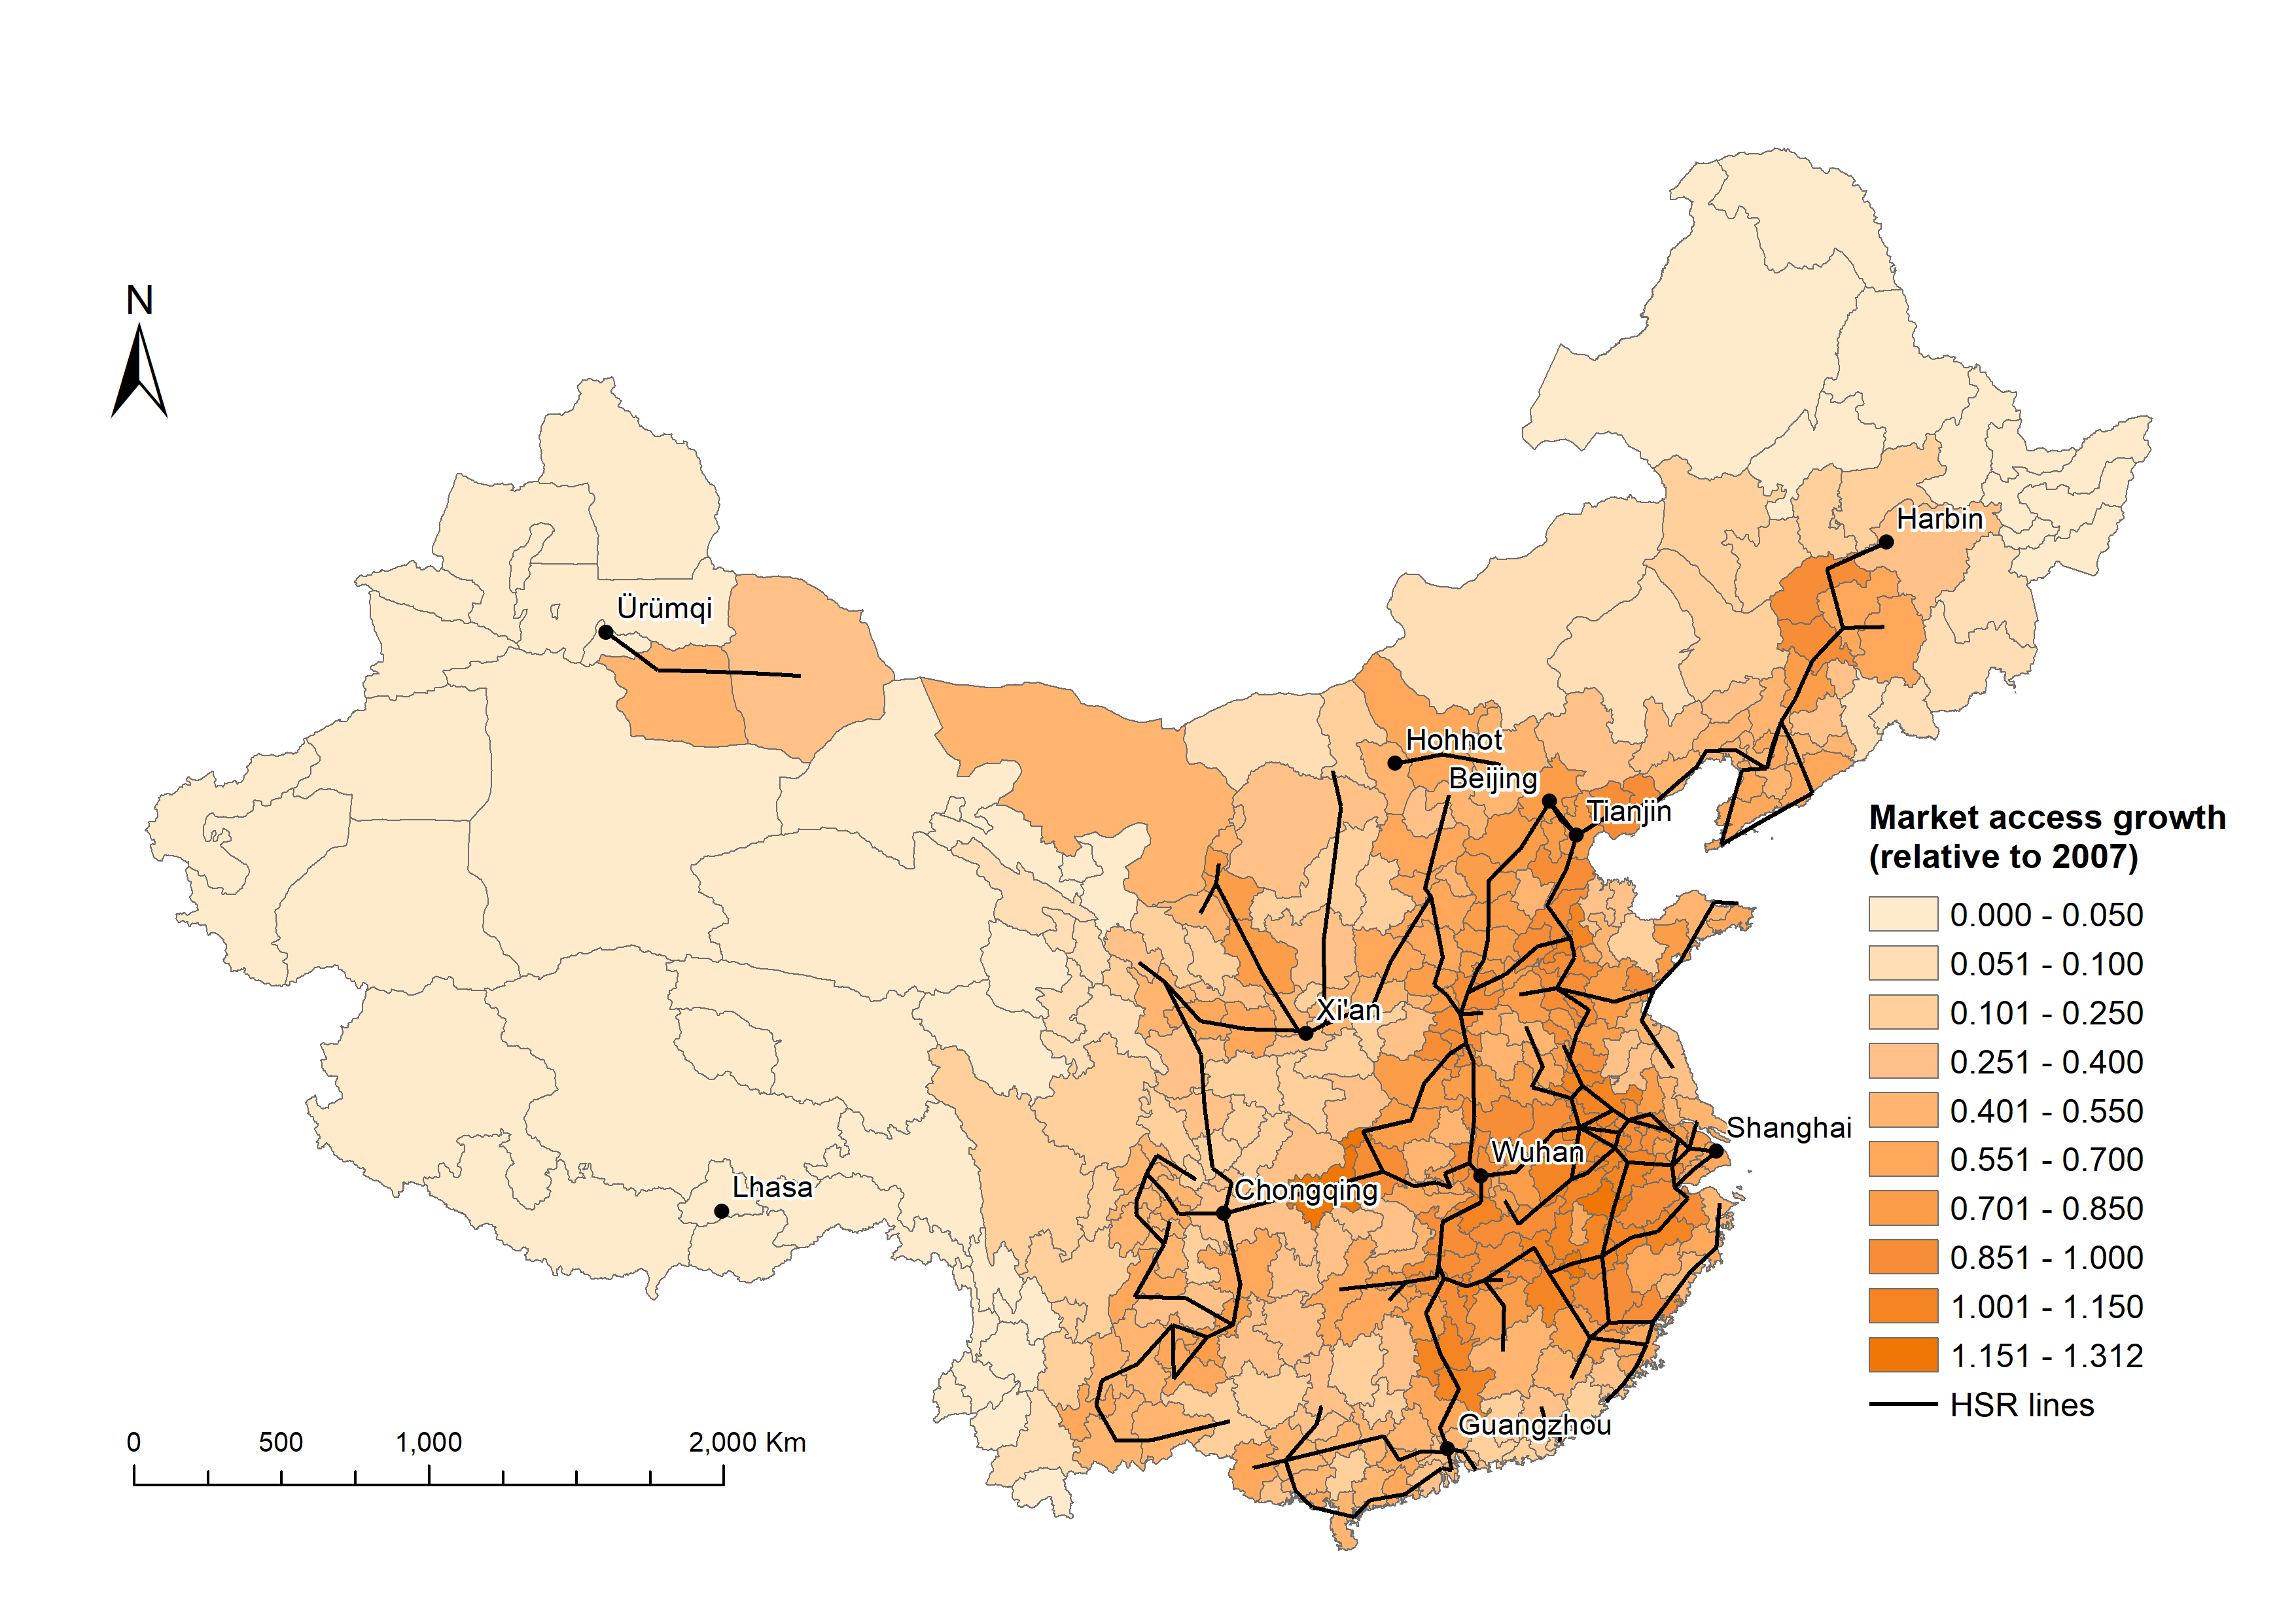
\includegraphics[trim={1cm 0.5cm 0.5cm 1cm},clip,width=11cm]{lecture_includes/Sim_Line_nlink2016.png}
	\end{center}
\end{frame}

\begin{frame}[t]{Illustration: High-Speed Rail in China} 
\vspace{-0.3cm}
	\begin{center}
		Expected MA growth, $\mu_i$

		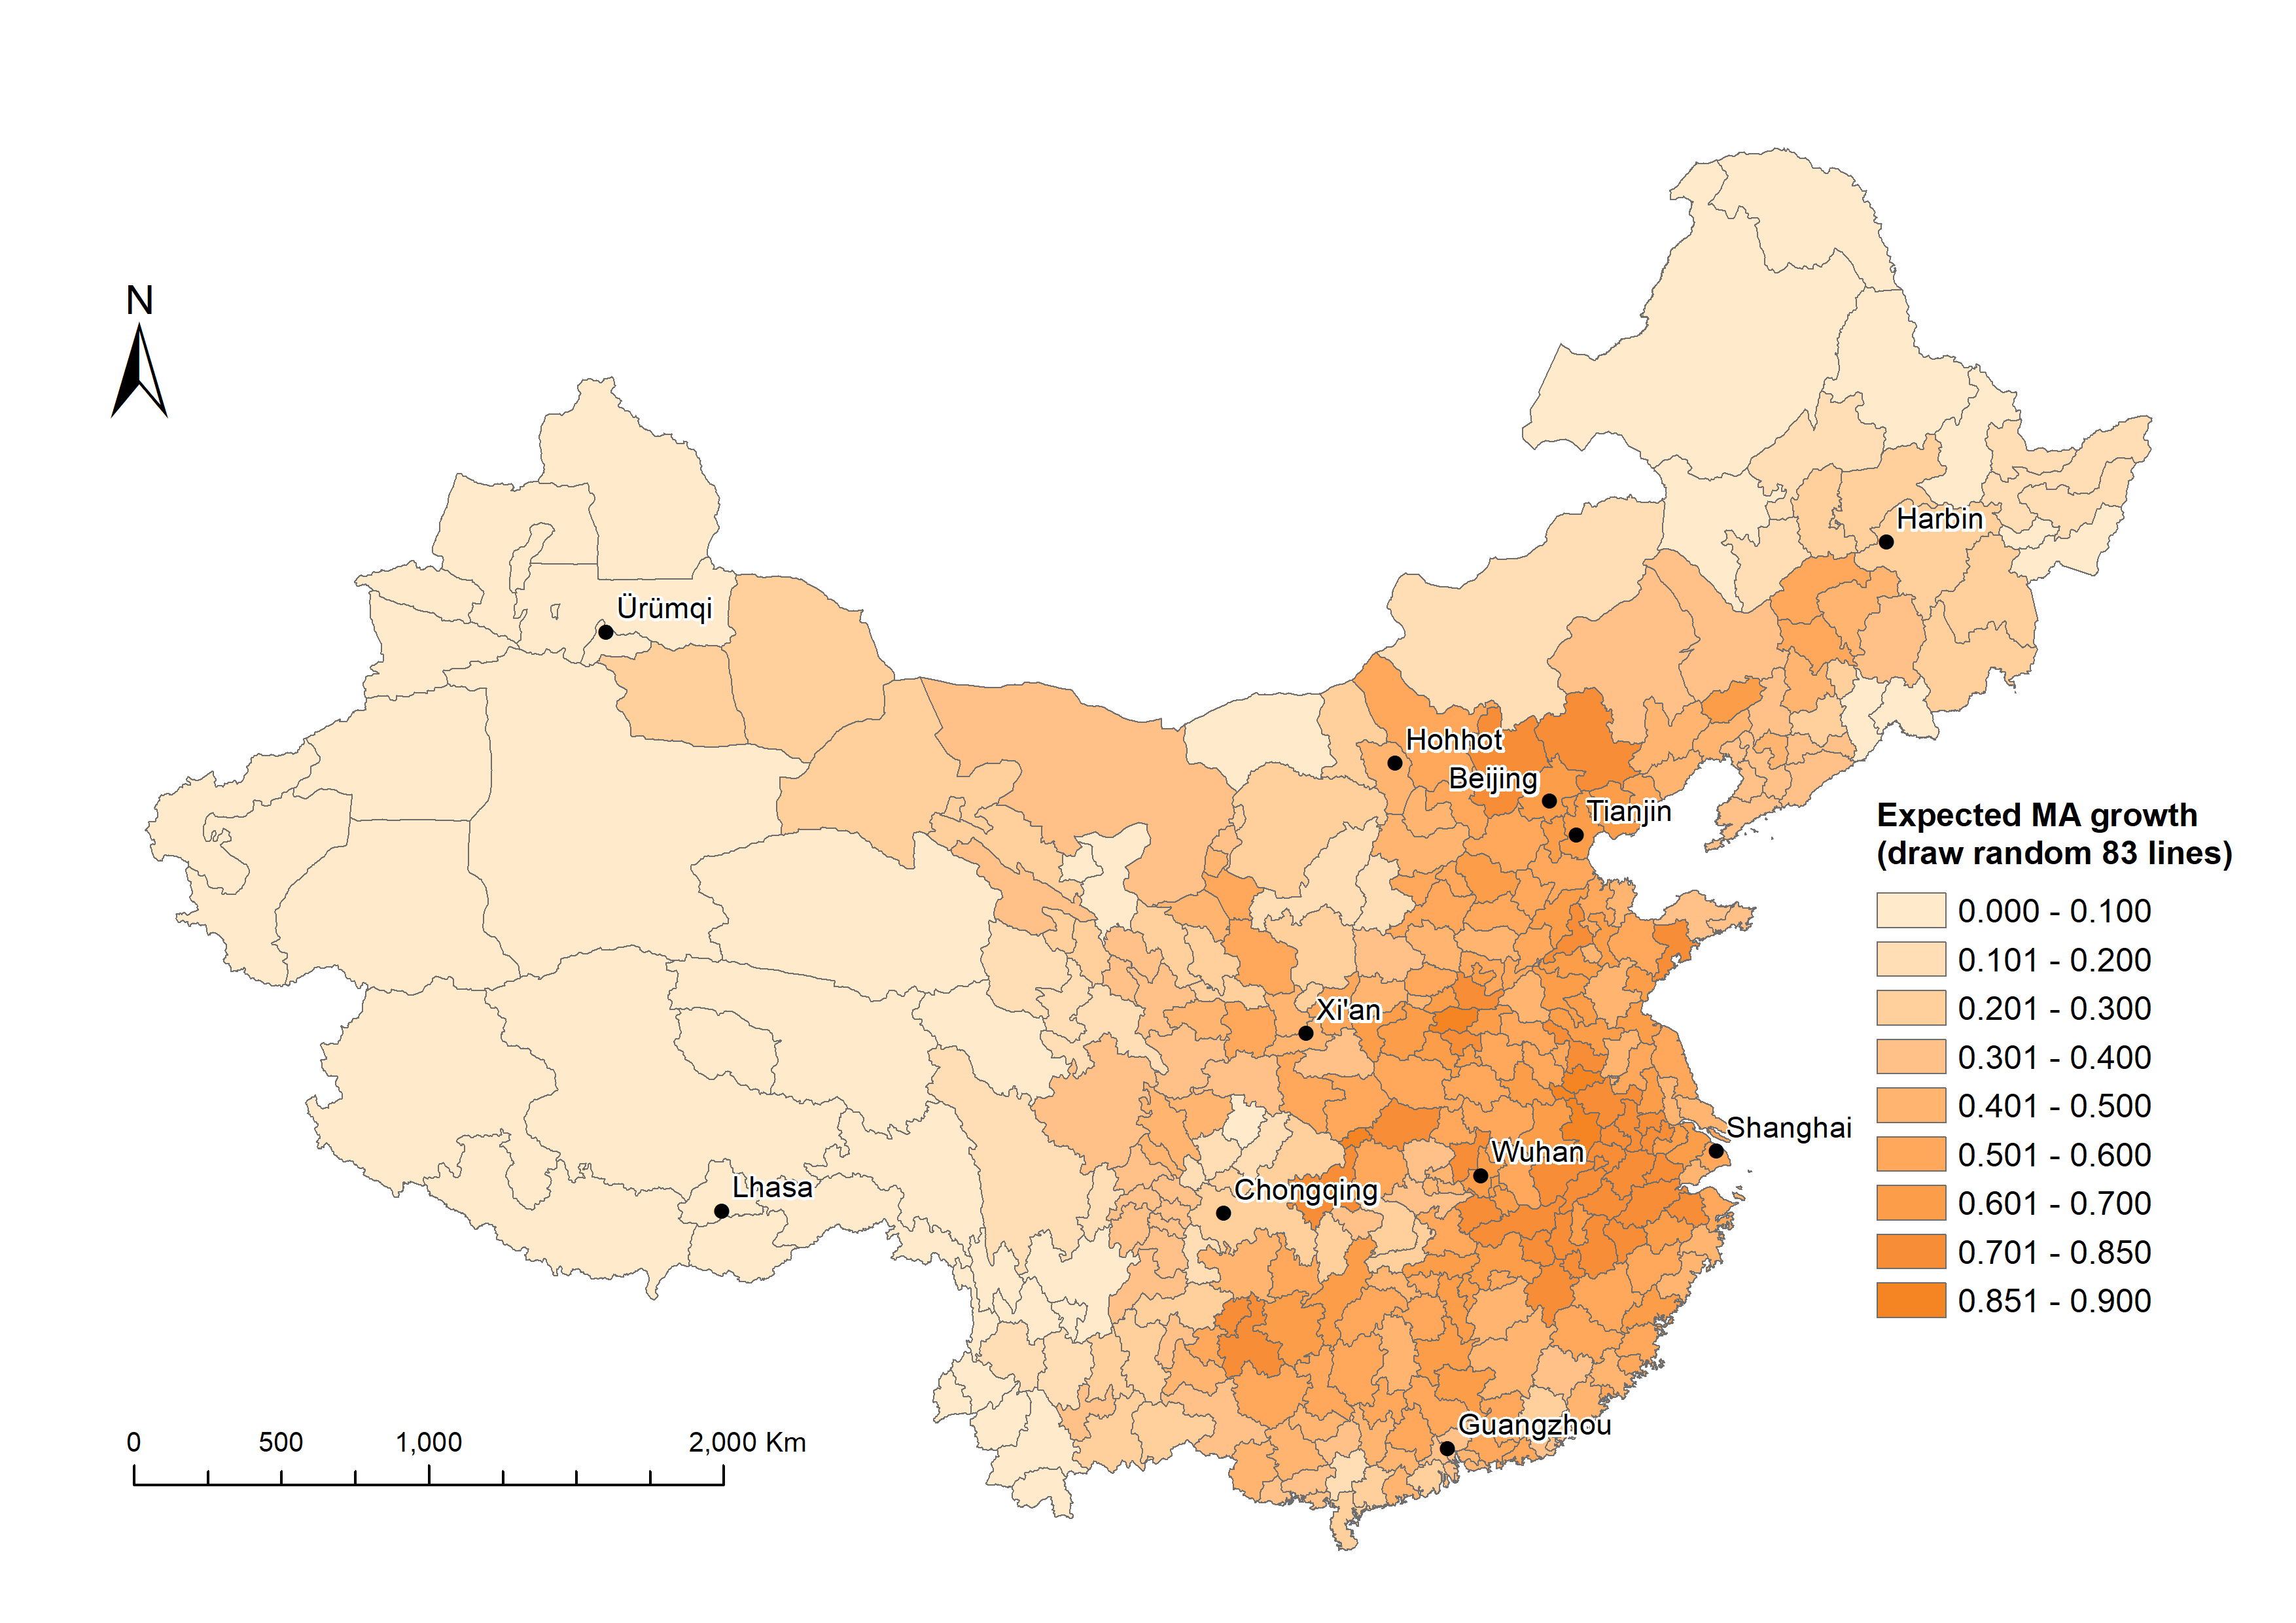
\includegraphics[trim={1cm 0.5cm 0.5cm 1cm},clip,width=11cm]{lecture_includes/DateExpected2016.png}
	\end{center}
\end{frame}

\begin{frame}{Illustration: High-Speed Rail in China}
	\begin{center}
Recentered MA growth, $Z_i$

	\includegraphics[trim={1cm 0.5cm 0cm 1cm},clip,width=11cm]{lecture_includes/NlinkRecentered2016.png}
	\end{center}
\end{frame}

\begin{frame}[label=HSRTable]{Adjusted Estimates of Market Access Effects}
	\begin{center}
	\includegraphics[width=0.9\textwidth]{lecture_includes/hsr_tab.png}
	
	\footnotesize{Regressions of log employment growth on log market access growth in 2007--2016. Spatial-clustered standard errors in parentheses; permutation-based 95\% CI in brackets}
	\end{center}
\end{frame}

\begin{frame}{Recentering for Power}

Leveraging non-random exposure can dramatically improve precision when leveraging exogenous shocks in an IV...
\begin{itemize}
\item ... as long as you recenter to use this variation ``safely''
\end{itemize}\medskip\pause{}

Ex: Medicaid eligibility s a treatment combining statewide policy shocks and individual exposure (income, family structure, etc)
\begin{itemize}
\item In settings where policy shocks are plausibly exogenous, standard approach is to use them directly as instruments (``simulated IV'')
\item BH approach: use eligibility itself, but recenter: e.g. adjust for $i$'s avg. eligibility across permutations of policies (swap MA \& RI, say)
\end{itemize}

\end{frame}

\begin{frame}{Illustration: ACA Medicaid Expansion}

	\begin{center}
	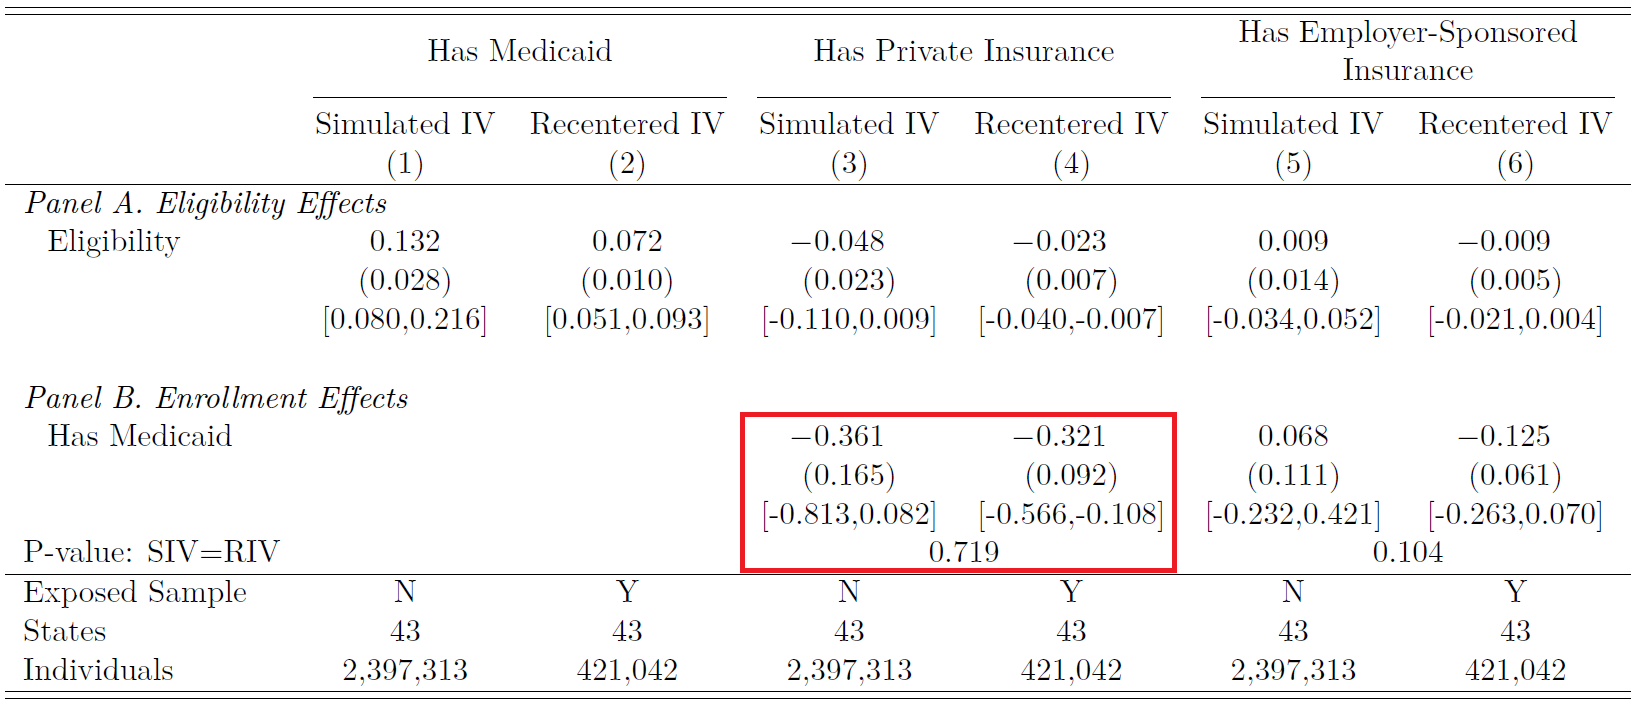
\includegraphics[width=1\textwidth]{lecture_includes/aca_ss.png}
	\end{center}

\footnotesize{1\% ACS sample of non-disabled adults in 2013--14, diff-in-diff IV regressions using one of the two instruments. Controls include state and year fixed effects and an indicator for Republican governor interacted with year. State-clustered standard errors in parentheses; wild score bootstrap 95\% CI in brackets} 

\end{frame}

\begin{frame}{Concluding Thoughts}

We've covered a ton of ground in two days! 
\begin{itemize}
\item From basic IV mechanics to advanced recentering techniques
\end{itemize}\bigskip\pause{}

Some general advice on how to approch IV in the ``real world'':
\begin{enumerate}
\item Figure out what the reduced form and first stage regressions are, \\ \& what variation in the instrument(s) they leverage via the controls
\item Assess the plausibility of as-good-as-random assignment (or parallel trends) of this variation, both theoretically and empirically
\item Interrogate exclusion, which lets you interpret RF/FS, and monotonicity/complier stats if heterogeneous FX seem important
\end{enumerate}
\end{frame}

\begin{frame}{Keep Calm and \code{ivreg2} On!}

\begin{center}
Thank you, and good luck on your future adventures with IV!

\bigskip
\url{peter_hull@brown.edu}

\end{center}
\end{frame}
\end{document}
